\chapter{A Flagship Space Telescope Opening Korea's Space Era}

Over the past decade, the landscape of space-based astronomy has undergone a profound transformation. The traditional paradigm of large flagship missions characterized by long development cycles and high costs has gradually shifted toward a model emphasizing shorter development times, focused instrument capabilities, and rapid responsiveness to time-critical scientific observations. This transition is closely associated with the evolving observational requirements of key areas in modern astrophysics, including gravitational-wave and neutrino astronomy, time-domain astrophysics, and exoplanet research [1,2].

The 3.5-meter Segmented-Mirror Robotic Space Telescope has been conceived within this international context as a nationally led space astronomy infrastructure aimed at establishing Korea's independent space-based observational capability and advancing the nation toward a leading position in space science. The mission has two primary objectives. First, it seeks to secure high-precision and highly stable optical and near-infrared observational capabilities that cannot be fully achieved through ground-based observations. Second, it aims to realize an efficient and sustainable space telescope capable of delivering high scientific impact within a realistic development schedule and budget, compared to conventional large flagship missions [4,5].

The telescope combines a 3.5-meter-class segmented primary mirror, active wavefront control technology, and a highly automated robotic observing and operational framework. This design is optimized for time-domain and multi-messenger astronomy, where rapid target acquisition and prompt follow-up observations are essential. Consequently, the observatory will serve as a valuable asset within international observing networks for the study of gravitational-wave events, gamma-ray bursts, rapidly evolving supernovae and variable objects, and near-Earth objects (NEOs) requiring urgent and high-priority observations [1,6].

Furthermore, the mission is designed not as a standalone facility but as part of a broader observational ecosystem that includes future ground-based large telescopes, next-generation space observatories, and international time-domain survey projects. Through such integration, Korean researchers will be able to participate proactively in major international scientific programs from their early stages, while accumulated operational experience and technological expertise can be leveraged to support future space astronomy missions [8,9].

Beyond its scientific capabilities, the 3.5-meter Segmented-Mirror Robotic Space Telescope carries significant symbolic importance as Korea's first large-aperture space telescope to be independently designed, developed, and operated. The mission will elevate the maturity of the nation\textquotesingle s space science and technology capabilities while serving as a technological and scientific stepping stone toward future flagship-class space observatories [5,7].

Under these objectives, this paper is organized as follows. Chapter 2 presents the scientific motivations and key scientific questions. Chapter 3 describes the mission design principles. Chapter 4 introduces the telescope architecture and system configuration. Chapter 5 discusses the expected scientific outcomes. Chapter 6 outlines the operational concept, including orbital considerations, rapid-response observations, and the data and community-utilization strategy. Chapter 7 concludes by placing the proposed telescope within the future domestic and international space astronomy landscape.

\chapter{Science Motivation}

The 3.5-meter Segmented-Mirror Robotic Space Telescope aims to establish a core space-based observational capability that will enable the Republic of Korea to respond proactively to the rapidly evolving landscape of modern astronomical research. This objective is well aligned with the Fourth Basic Plan for the Promotion of Space Development and is intended to complement the capabilities of existing and planned astronomical facilities. Contemporary astronomy is increasingly driven by wide-field surveys, multi-messenger observations, and time-domain astrophysics, creating a growing demand for facilities that can simultaneously provide rapid response, operational flexibility, and highly stable spectroscopic and imaging performance. These scientific requirements are difficult to satisfy through either single-purpose flagship missions or ground-based observations alone, making large-aperture space telescopes operated in the stable environment of space increasingly important for future astronomical research [1,2,3].

By combining a 3.5-meter-class segmented primary mirror, active wavefront control technology, and a highly automated robotic operational concept, the proposed telescope is designed as a versatile platform capable of conducting both time-critical observations and long-term precision investigations. The mission is intended to play a complementary role alongside existing and planned domestic and international observatories while also serving as a scientific and technological pathfinder for future flagship-class space astronomy missions. In particular, the telescope carries strategic significance in that it will provide Korean researchers with the capability to participate in international observational networks not merely as contributing partners, but as stakeholders possessing a key scientific asset and observational resource [5,7].

\section{Cosmology}

Cosmology is one of the central fields of modern astrophysics, aiming to understand the origin and evolution of the Universe as well as the nature of dark energy and dark matter. Observational discoveries over the past several decades have provided compelling evidence that the Universe is undergoing accelerated expansion, leading to the introduction of dark energy as a fundamental component of the standard cosmological model [8,9,10]. Despite its success in explaining a wide range of observations, the physical origin and properties of dark energy remain largely unknown. Moreover, subtle but statistically significant tensions have emerged among cosmological parameters derived from different observational techniques, raising important questions about our current understanding of the Universe [8].

Addressing these issues requires independent observational methods capable of cross-validating cosmological parameters. Various probes, including Type Ia supernovae, gravitational-wave standard sirens, galaxy clusters, and weak gravitational lensing, have been employed for this purpose. Many of these approaches rely on high-precision photometric and spectroscopic observations in the optical and near-infrared wavelength ranges. However, ground-based observations are fundamentally limited by atmospheric effects and changing observing conditions, which introduce systematic uncertainties and constrain the long-term stability and absolute precision required for precision cosmology.

Operating in the stable environment of space, the 3.5-meter Segmented-Mirror Robotic Space Telescope will provide repeated and homogeneous observations of Type Ia supernovae and other potential standard candles. Its time-domain observing capability will enable continuous monitoring from the earliest phases immediately following an explosion through the long-term fading stage. Such observations will improve our understanding of the relationship between supernova physics and cosmological distance measurements, thereby refining the cosmic distance scale. Beyond improving distance measurement accuracy, these data will also help identify and characterize the physical origins of systematic uncertainties associated with supernova-based cosmology [1,11].

In addition, the telescope will observe electromagnetic counterparts associated with gravitational-wave events, enabling independent cosmological constraints based on standard sirens. Because such measurements are independent of the traditional electromagnetic distance ladder, they offer a powerful means of investigating the currently reported Hubble constant tension and potentially identifying its underlying cause. These observations require both rapid-response capability and stable spectroscopic performance, making them directly aligned with the primary design objectives of the 3.5-meter space telescope.

\section{Galaxies}

The formation and evolution of galaxies result from the complex interplay of star formation, gas accretion and circulation, and the growth of supermassive black holes. These processes operate over a wide range of timescales throughout cosmic history and leave observable signatures in galaxy morphology, color, chemical composition, and nuclear activity. A central goal of galaxy evolution studies is to establish the physical connections between these observable properties and the underlying astrophysical processes that drive them.

The optical and near-infrared wavelength ranges provide the most direct means of tracing stellar populations, interstellar gas, and galactic structures. However, ground-based observations are limited by atmospheric emission, absorption, and seeing effects, which hinder precise measurements of fine structural features and faint low-surface-brightness components. In particular, systematic investigations of galaxy outskirts, diffuse low-surface-brightness structures, and the complex environments surrounding galactic nuclei are difficult without space-based observations.

With its near-diffraction-limited spatial resolution and stable spectroscopic performance, the 3.5-meter Segmented-Mirror Robotic Space Telescope will enable detailed studies of the structure and physical properties of nearby and intermediate-redshift galaxies [9]. By simultaneously tracing star-forming regions, gas distributions, and the variability characteristics of active galactic nuclei (AGNs), the telescope will provide direct observational constraints on the energy feedback mechanisms that regulate galaxy evolution. In particular, time-domain observations of AGN variability will offer valuable insights into the connection between black hole growth and the evolutionary pathways of galaxies.

Furthermore, the telescope will play a key role in international collaborative research by providing deeper and more precise follow-up observations of targets selected from large-scale ground-based survey programs. Such capabilities will enhance both the visibility and scientific leadership of Korean researchers in the field of galaxy evolution studies.

\section{Compact Objects}

Compact objects provide natural laboratories for studying the behavior of matter and energy under extreme conditions of gravity, density, and magnetic fields. The simultaneous observation of gravitational waves and electromagnetic signals from neutron star and black hole mergers has become one of the fastest-growing fields in modern astrophysics [1].

These events typically undergo rapid physical evolution over very short timescales, with the earliest phases containing critical information about the underlying physical processes. However, currently operating large space telescopes often face scheduling constraints that limit their ability to respond immediately to such transient phenomena. Ground-based telescopes, while capable of rapid follow-up observations, are subject to atmospheric conditions and interruptions caused by the day--night cycle.

The 3.5-meter Segmented-Mirror Robotic Space Telescope is designed to initiate observations within a few hours of receiving a gravitational-wave alert. This capability will enable detailed studies of the early spectral evolution of kilonovae, high-energy emission mechanisms, and the nucleosynthesis of heavy elements. Combined with long-term time-series observations, the telescope will also be able to trace the cooling and recombination processes of merger remnants over extended periods.

Such observations are essential for constraining the equation of state of ultra-dense matter, understanding the formation of relativistic jets, and investigating radiative processes in extreme gravitational environments. The proposed telescope will provide the capabilities necessary to serve as a key component of the international observational network dedicated to multi-messenger studies of compact objects.

\section{Exoplanets}

Exoplanet research has transitioned from the discovery phase to the characterization phase, with current efforts focused on understanding the physical and chemical properties of planetary atmospheres [12]. Achieving this goal requires highly stable photometric and spectroscopic observations capable of accurately correcting for stellar variability and activity, which can significantly affect atmospheric measurements.

Space-based observations provide the optimal environment for meeting these requirements. Through transit spectroscopy and long-term photometric monitoring, the 3.5-meter Segmented-Mirror Robotic Space Telescope will enable systematic investigations of exoplanet atmospheric composition, cloud properties, and star--planet interactions. In particular, repeated observations of small- and intermediate-sized planets will play a crucial role in improving the reliability and statistical significance of detected atmospheric signals.

In addition, the mission will employ high-contrast observational techniques to conduct direct investigations of selected nearby planetary systems, thereby enhancing the technological and scientific readiness for future life-detection and habitable-world exploration missions. This approach provides a strategic pathway that simultaneously delivers near-term scientific achievements while contributing to the long-term goals of space exploration and the search for life beyond the Solar System.

\section{Near-Earth Objects}

Near-Earth Objects (NEOs) are remnants of the formation and evolution of the Solar System and, at the same time, represent potential impact hazards to Earth [13]. Accurate determination of their orbital parameters and physical properties is therefore important not only for scientific investigations but also for planetary defense and public safety.

Ground-based survey programs have successfully discovered a large number of NEOs; however, refining their orbital elements and characterizing their physical properties often require additional space-based observations. Through repeated astrometric measurements and spectroscopic observations, the 3.5-meter Segmented-Mirror Robotic Space Telescope will significantly improve the accuracy of orbit determination and long-term trajectory predictions [14].

The mission is designed to operate in close coordination with international planetary defense networks, playing a critical role throughout the entire process of discovery, tracking, and physical characterization of potentially hazardous objects. As such, the telescope will represent a compelling example of how a Korean space observatory can contribute not only to fundamental scientific research but also directly to the safety and well-being of human society.

\chapter{Mission Design Guidelines}

\section{Fundamental Philosophy of Mission Design}

The mission design of the 3.5-meter Segmented-Mirror Robotic Space Telescope is not aimed merely at realizing a telescope that satisfies a specific set of performance metrics. Rather, the primary goal of this mission is to develop a space telescope capable of providing the most scientifically needed observations at the most appropriate time within the rapidly evolving astronomical research environment of the 2030s and beyond.

Contemporary astronomy is rapidly transitioning into a network-based science that integrates wide-field surveys, time-domain observations, and multi-messenger astronomy. In this environment, the success of an observation is determined not only by maximizing a single performance parameter, but also by rapid response, stability, repeatability, and connectivity with international observing networks. In this respect, the present mission treats schedule, operations, and system architecture as design variables of equal importance to the scientific objectives themselves.

Against this background, this section presents the high-level principles and specific guidelines required to realize the scientific motivations defined above. These guidelines are not intended simply to list performance requirements. Rather, by clearly defining what choices will be made and what choices will not be pursued, they serve to systematically control scope expansion and risk escalation during the development process.

\section{Level-0 Mission Objectives}

\subsection{Realization of a Large-Aperture Space Telescope Led by the Republic of Korea}

The first Level-0 objective of the mission is to realize a large-aperture (3.5-meter-class) optical--near-infrared space telescope that can be independently designed, developed, and operated by the Republic of Korea. This objective extends beyond technology demonstration or the development of individual subsystems. It encompasses the establishment of national capabilities for the integrated design, implementation, and operation of an entire space telescope system, including the optical assembly, structural system, attitude control, thermal control, science operations, and data processing infrastructure.

The 3.5-meter segmented-mirror architecture represents a practical yet ambitious solution that overcomes launch vehicle constraints while providing light-gathering power and angular resolution exceeding those of the Hubble Space Telescope. Through this mission, Korea will establish the capability to conduct long-term, highly stable, and high-precision observations in the space environment free from atmospheric limitations.

\subsection{Addressing the Observational Gap in the Scientific Landscape of the 2030s}

The second Level-0 objective is to address the anticipated gap in large-aperture space-based observations in the optical and near-infrared wavelength ranges following the gradual retirement of the Hubble Space Telescope. While the James Webb Space Telescope (JWST) is optimized for near- and mid-infrared observations, its observing model and exceptionally high demand impose inherent limitations on rapid-response and highly flexible observational programs.

In this context, the proposed mission aims to serve as a highly stable, rapid-response observing platform in the optical and near-infrared regime and to become a key asset within the international astronomical observing network. Such a capability would enable Korean scientists to participate in major international scientific programs not merely as users or collaborators, but as providers of a critical observational resource, thereby establishing a new framework for scientific leadership and international partnership.

\section{Key Mission Design Principles}

\subsection{Schedule-Driven Desig}

Rather than pursuing the highest achievable performance at any cost, this mission adopts as its starting point the realization of a telescope that can be deployed when its scientific impact will be greatest. Development schedule is therefore treated not merely as an administrative constraint but as a fundamental design parameter that directly influences scientific return.

To support this approach, mission requirements are clearly defined and frozen at an early stage of development, and scope expansion during implementation is subject to strict control. Any proposed enhancement in functionality or performance must be evaluated against four key criteria: scientific impact, schedule delay, cost increase, and risk escalation. Only modifications that demonstrate a favorable balance among these factors should be considered for incorporation into the mission baseline.

\subsection{Managed Risk Acceptance}

A 3.5-meter segmented-mirror space telescope inherently involves significant technological challenges. However, the mission does not follow the traditional flagship philosophy of attempting to eliminate all risks prior to implementation. Instead, it adopts a strategy of explicitly identifying risks and accepting them within carefully managed and well-defined boundaries.

This approach prioritizes the use of proven technologies whenever possible, while concentrating development efforts on the mission-critical elements that determine overall performance, including segmented-mirror alignment, active wavefront control, and high-stability attitude control. Risks associated with these key technologies are mitigated through a phased development process involving incremental demonstrations, subsystem validation, and iterative testing.

By balancing innovation with risk management, this strategy provides a practical pathway toward achieving significant scientific capability while maintaining control of development costs and schedule. It represents a realistic compromise between technological ambition and programmatic sustainability, enabling the mission to deliver substantial scientific return without the excessive complexity often associated with large flagship observatories.

\subsection{Elevating Rapid Response to a Core Mission Requirement}

In this mission, rapid response is not regarded as an optional operational capability but as a fundamental requirement that shapes the entire mission architecture. For transient phenomena such as gravitational-wave events, supernova explosions, and rapidly evolving astrophysical sources, delays in observation can directly translate into the loss of unique scientific opportunities.

Accordingly, rapid-response capability is defined as an end-to-end system requirement encompassing the attitude control system, observation scheduler, ground-segment operations, data-processing pipeline, and operational staffing framework. This principle establishes the robotic operational concept as a defining characteristic of the mission and a central element of its scientific identity.

\subsection{Focused Instrumentation and a Clear Mission Identity}

The mission is not intended to incorporate the widest possible range of observational modes. Instead, it adopts a focused instrument suite optimized for addressing the key scientific objectives defined in Chapter 2.

Optical--near-infrared imaging, spectroscopy, and high-cadence time-series photometry are designated as the core observational capabilities of the mission. Additional functionalities will be considered only after careful evaluation of their impacts on schedule, cost, technical risk, and overall mission effectiveness. This approach is intended to avoid unnecessary complexity that could dilute the mission's scientific identity, while maximizing both development efficiency and operational effectiveness.

\subsection{Complementary Network-Centric Design}

The mission is not intended to replace existing or planned domestic and international astronomical facilities. Instead, it is designed to occupy the observational niche where space-based, highly stable, and rapid-response observations provide the greatest value within the scientific workflow of discovery, follow-up characterization, and precision monitoring.

Through this approach, the telescope will function as a network-centric space observatory that naturally complements ground-based wide-field survey facilities, gravitational-wave detectors, and future space missions. By operating as an integral component of a broader international observational ecosystem, the mission will maximize its scientific impact while enhancing global collaboration and observational synergy.

\subsection{Deliberate Preservation of Versatility and Expandability}

The mission design is not optimized exclusively for a limited set of predefined scientific cases. Instead, it intentionally preserves flexibility in observational modes and operational policies to ensure that the telescope can address new scientific questions that may emerge during its anticipated operational lifetime of more than two decades.

This principle is essential for maximizing the long-term scientific value of the mission and ensuring its role as a lasting scientific legacy observatory capable of supporting discoveries beyond those envisioned at the time of its design.

\subsection{Iterative and Agile Systems Engineering Approach}

The mission adopts an iterative systems engineering methodology rather than a strictly linear development model. Throughout the Development Model (DM), Engineering Model (EM), Qualification Model (QM), and Flight Model (FM) phases, repeated sensitivity analyses are performed to evaluate the interactions among scientific requirements, system performance, cost, and risk. This process enables mission design decisions to be progressively refined as the project matures.

Such an approach allows technological maturity and scientific requirements to evolve in parallel, reducing the likelihood that early design choices will impose irreversible constraints or introduce mission-critical vulnerabilities. By continuously reassessing key trade-offs throughout development, the mission can maintain both technical robustness and scientific relevance.

\section{Summary of the Mission Design Guidelines}

In summary, the mission design guidelines for the 3.5-meter Segmented-Mirror Robotic Space Telescope can be summarized as follows:

\begin{enumerate}
\def\labelenumi{\arabic{enumi}.}
\item
  \textbf{Timeliness-Driven Design}\\
  The scientific value of the mission depends not only on what the telescope can do, but also on when it becomes operational.
\item
  \textbf{Managed Risk Acceptance}\\
  Risks are explicitly identified, assessed, and managed in a structured and transparent manner rather than being concealed or avoided entirely.
\item
  \textbf{System-Level Integration of Rapid Response Capability}\\
  Rapid-response operation is established as a core mission requirement, with robotic operations serving as a defining feature of the observatory.
\item
  \textbf{Focus and Discipline}\\
  The mission concentrates on the minimum set of essential capabilities required to achieve its primary scientific objectives while avoiding unnecessary complexity.
\item
  \textbf{Network-Centric Perspective}\\
  The mission seeks to maximize international scientific synergy and collaborative impact rather than pursuing isolated achievements.
\item
  \textbf{Long-Term Scientific Legacy}\\
  The telescope is designed not only to address today\textquotesingle s scientific questions but also to remain adaptable to the unforeseen discoveries and research challenges of the future.
\end{enumerate}

\chapter{Space Telescope Architecture \& Design Capabilities}

\section{Telescope Overview}

\begin{figure}[htbp]\centering
  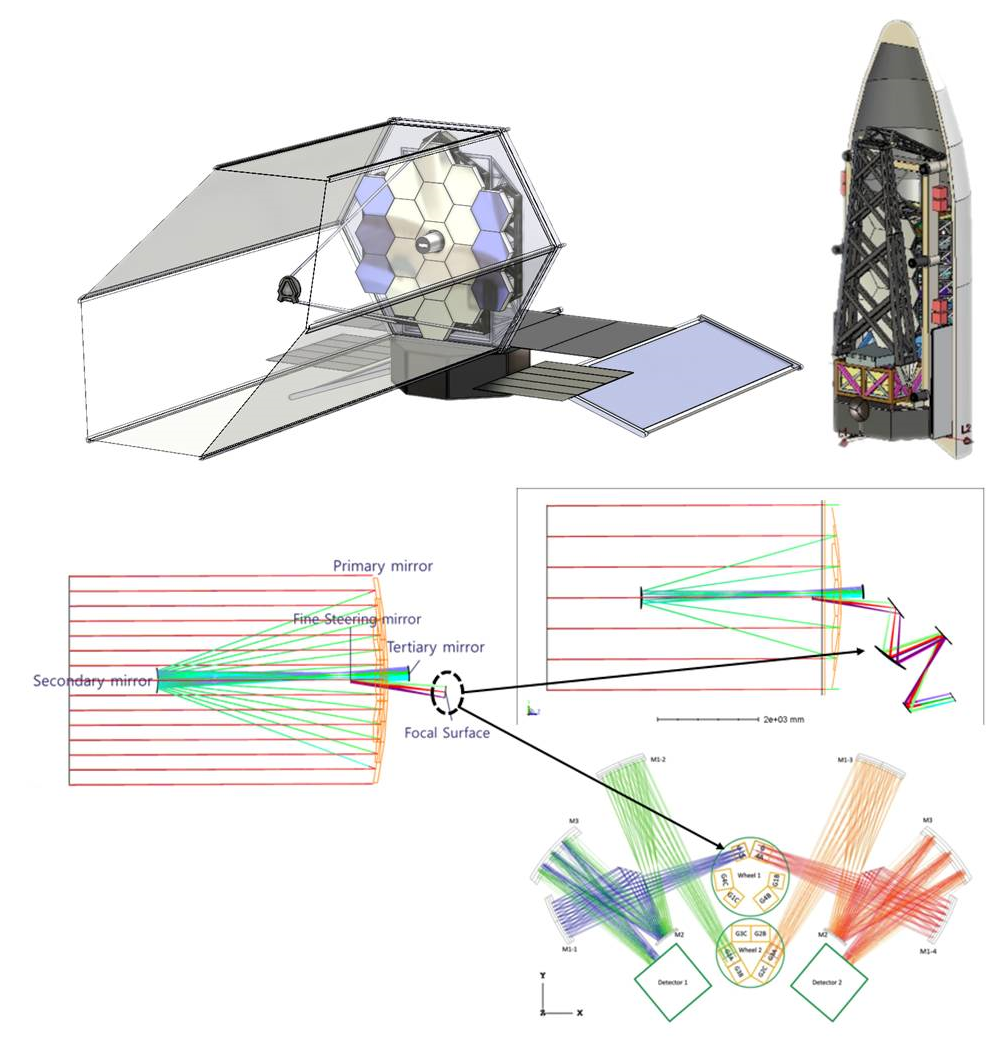
\includegraphics[width=0.85\linewidth,height=0.42\textheight,keepaspectratio]{book_media/image1.png}
\end{figure}

Fig. 1. Schematic diagram of the 3.5-meter segmented-mirror robotic space telescope and its UV, VIS, and IR instruments

\textbf{Table 1}. Basic Specifications of the 3.5 m Segmented-Mirror Robotic Space Telescope

\begin{longtable}[]{@{}
  >{\raggedright\arraybackslash}p{(\columnwidth - 4\tabcolsep) * \real{0.3336}}
  >{\raggedright\arraybackslash}p{(\columnwidth - 4\tabcolsep) * \real{0.1083}}
  >{\raggedright\arraybackslash}p{(\columnwidth - 4\tabcolsep) * \real{0.5581}}@{}}
\toprule\noalign{}
\multicolumn{2}{@{}>{\raggedright\arraybackslash}p{(\columnwidth - 4\tabcolsep) * \real{0.4419} + 2\tabcolsep}}{%
\begin{minipage}[b]{\linewidth}\raggedright
\textbf{Parameter}
\end{minipage}} & \begin{minipage}[b]{\linewidth}\raggedright
\textbf{Specification}
\end{minipage} \\
\midrule\noalign{}
\endhead
\bottomrule\noalign{}
\endlastfoot
Optical Configuration & \multicolumn{2}{>{\raggedright\arraybackslash}p{(\columnwidth - 4\tabcolsep) * \real{0.6664} + 2\tabcolsep}@{}}{%
3.5 m segmented-mirror on-axis optical system

using 18 hexagonal mirror segments} \\
Primary Mirror Diameter & \multicolumn{2}{>{\raggedright\arraybackslash}p{(\columnwidth - 4\tabcolsep) * \real{0.6664} + 2\tabcolsep}@{}}{%
3.5 m} \\
Focal Ratio & \multicolumn{2}{>{\raggedright\arraybackslash}p{(\columnwidth - 4\tabcolsep) * \real{0.6664} + 2\tabcolsep}@{}}{%
f/4.5} \\
Wavelength Range & \multicolumn{2}{>{\raggedright\arraybackslash}p{(\columnwidth - 4\tabcolsep) * \real{0.6664} + 2\tabcolsep}@{}}{%
0.2 μm -- 3.0 μm} \\
Field of View & \multicolumn{2}{>{\raggedright\arraybackslash}p{(\columnwidth - 4\tabcolsep) * \real{0.6664} + 2\tabcolsep}@{}}{%
10′×10′--30'×30′} \\
Instruments & \multicolumn{2}{>{\raggedright\arraybackslash}p{(\columnwidth - 4\tabcolsep) * \real{0.6664} + 2\tabcolsep}@{}}{%
Imaging camera (Ultraviolet--Visible--Infrared, UVOIR),

spectrograph (UVOIR), stellar coronagraph} \\
Angular Resolution & \multicolumn{2}{>{\raggedright\arraybackslash}p{(\columnwidth - 4\tabcolsep) * \real{0.6664} + 2\tabcolsep}@{}}{%
UV/Visible: 0.03″, Near-Infrared: 0.09″} \\
Sensitivity & \multicolumn{2}{>{\raggedright\arraybackslash}p{(\columnwidth - 4\tabcolsep) * \real{0.6664} + 2\tabcolsep}@{}}{%
Approximately 27.7 mag in the visible channel} \\
Observing Modes & \multicolumn{2}{>{\raggedright\arraybackslash}p{(\columnwidth - 4\tabcolsep) * \real{0.6664} + 2\tabcolsep}@{}}{%
Survey observations and pointed observations

(typical exposure time: \textasciitilde10 min)} \\
Pointing Accuracy/Stability & \multicolumn{2}{>{\raggedright\arraybackslash}p{(\columnwidth - 4\tabcolsep) * \real{0.6664} + 2\tabcolsep}@{}}{%
0.03″ / 10 min} \\
Orbit & \multicolumn{2}{>{\raggedright\arraybackslash}p{(\columnwidth - 4\tabcolsep) * \real{0.6664} + 2\tabcolsep}@{}}{%
Earth orbit or Sun--Earth L2 (Lagrange Point 2)} \\
Mission Lifetime & \multicolumn{2}{>{\raggedright\arraybackslash}p{(\columnwidth - 4\tabcolsep) * \real{0.6664} + 2\tabcolsep}@{}}{%
Baseline 10 years, with an additional 10 years

possible through robotic servicing missions} \\
Launch Vehicle Constraint & \multicolumn{2}{>{\raggedright\arraybackslash}p{(\columnwidth - 4\tabcolsep) * \real{0.6664} + 2\tabcolsep}@{}}{%
3 m fairing diameter} \\
\end{longtable}

The 3.5-meter Segmented-Mirror Robotic Space Telescope is a dedicated space observatory designed to perform highly stable, high-precision, and rapid-response observations in the optical and near-infrared wavelength ranges. By integrating a large-aperture segmented-mirror optical system, a high-precision attitude and pointing control system, and a robotic observing and operational concept, the telescope is designed to support both time-domain and multi-messenger astronomy as well as long-term precision monitoring programs.

At the core of the observatory is a 3.5-meter-class segmented primary mirror and the associated Optical Telescope Assembly (OTA) that supports it. Through the combination of active wavefront control and fine-pointing correction capabilities, the telescope aims to achieve image quality approaching the diffraction limit at optical wavelengths. Operating in an environment completely free from atmospheric disturbances, the observatory will provide the long-term observational stability required for scientific programs demanding exceptional photometric and spectroscopic precision.

The scientific payload is centered on wide-field imaging, precision time-series observations, and spectroscopic measurements. The entire observatory is designed around the capability for rapid target acquisition and the execution of highly automated observing sequences. As a result, the mission functions not merely as a single scientific instrument, but as an integrated observational platform capable of supporting a broad range of astrophysical investigations.

\section{Spacecraft Bus}\label{spacecraft-bus}

The scientific payload is integrated with a proven spacecraft bus that provides propulsion, attitude and orbit control, power generation and distribution, communications, and command and data handling functions. The bus design is based on technological heritage accumulated through previous space missions requiring deep-space operations and highly stable pointing performance. It incorporates the reliability and redundancy necessary for long-duration mission operations.

The attitude and pointing control system is designed as a multi-layer architecture to satisfy the stringent line-of-sight stability requirements imposed by the large-aperture optical system. High-precision pointing based on reaction wheels is combined with structural vibration minimization, passive and active vibration isolation, and fine-pointing correction mechanisms within the optical path. Together, these elements effectively suppress micro-vibrations and residual pointing errors during scientific observations.

The power subsystem employs fixed solar array panels to minimize the mechanical complexity and pointing disturbances associated with deployable structures. The thermal control system is primarily based on passive thermal management techniques designed to ensure the long-term stability of both the optical assembly and scientific instruments. Particular emphasis is placed on minimizing thermal fluctuations arising from the orbital environment and observing scenarios.

The communications and data handling system is designed to support highly automated mission operations and the transmission of large volumes of scientific data. Standardized data formats and interfaces with ground-segment infrastructure are incorporated from the outset to facilitate international collaborative observations and data sharing.

\section{Optical Telescope Assembly (OTA)}\label{optical-telescope-assembly-ota}

The Optical Telescope Assembly (OTA) is the core component that determines the scientific performance of the mission. The OTA is centered on a 3.5-meter-class segmented primary mirror and is designed to provide a large effective collecting area while satisfying launch vehicle fairing constraints. To achieve this objective, the primary mirror is composed of multiple mirror segments that are deployed and aligned to function as a single optical surface after launch.

\begin{figure}[htbp]\centering
  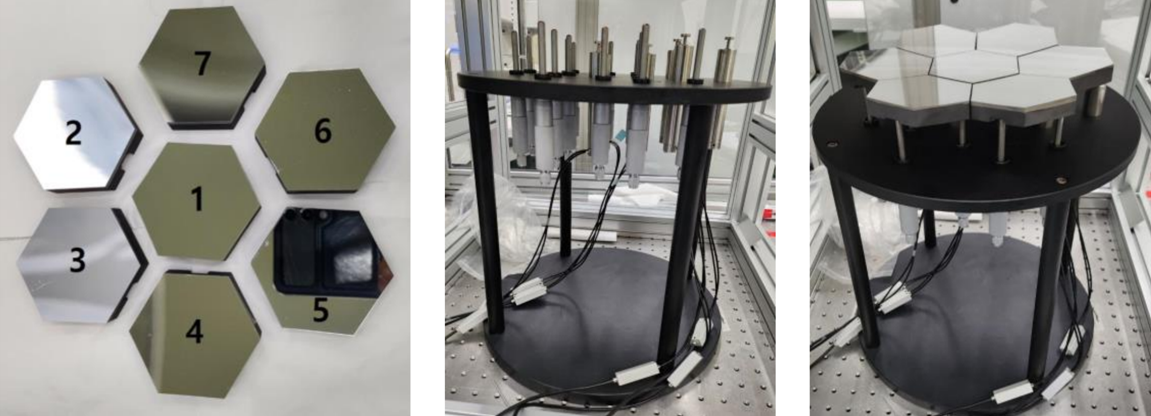
\includegraphics[width=0.85\linewidth,height=0.42\textheight,keepaspectratio]{book_media/image2.png}
\end{figure}

Fig. 2. Demonstration of segmented mirror phasing technology developed by KASI

The primary mirror segments are fabricated from lightweight, low-thermal-expansion materials and are designed to achieve optical performance equivalent to that of a monolithic mirror through active on-orbit alignment and wavefront correction. The active wavefront control system precisely regulates the relative positions and surface figures of the mirror segments, compensating for performance degradation caused by manufacturing tolerances, launch-induced disturbances, and thermally induced deformations.

The optical design is optimized to provide uniform image quality across a wide focal plane while simultaneously satisfying the requirements of multiple scientific instruments. The exit pupil and optical path incorporate a high-speed fine-steering element that provides fine-pointing correction, enabling the compensation of residual vibrations and pointing errors that occur during scientific observations.

The overall OTA design is intended to achieve three key objectives simultaneously: near-diffraction-limited optical performance, long-term thermal stability, and rapid thermal settling following target repointing maneuvers. These capabilities are essential for supporting both precision time-domain observations and long-duration scientific monitoring programs while maintaining consistent observational quality throughout the mission lifetime.

\begin{figure}[htbp]\centering
  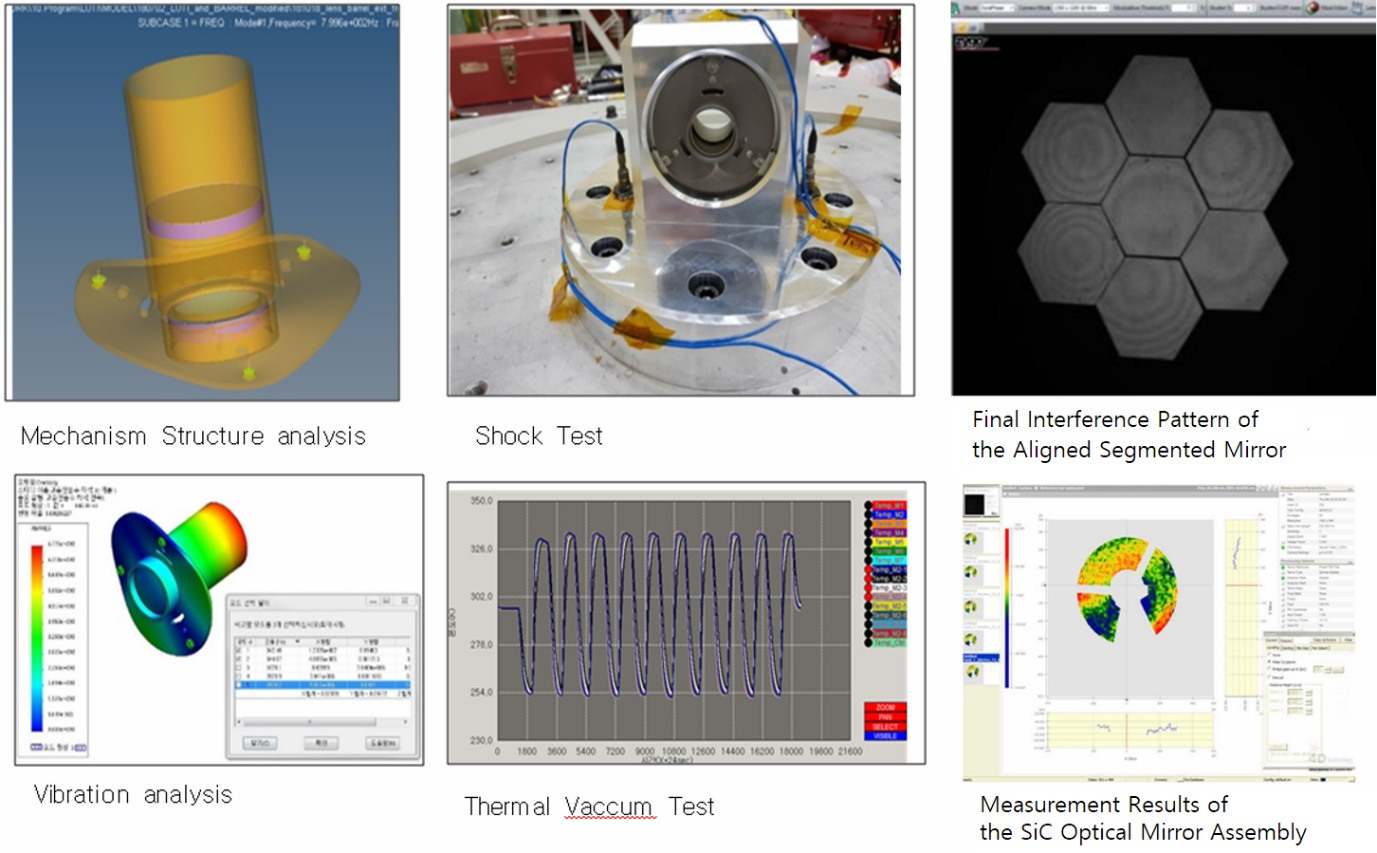
\includegraphics[width=0.85\linewidth,height=0.42\textheight,keepaspectratio]{book_media/image3.jpeg}
\end{figure}

Fig. 3. Attachment of fabricated segmented mirrors to the support structure, installation of actuators and micrometers, and alignment/control using an interferometer

\section{Wide-Field Imaging and Time-Domain Observation Instrument}\label{wide-field-imaging-and-time-domain-observation-instrument}

The Wide-Field Imaging Instrument serves as one of the primary scientific instruments of the mission, providing the core observational capability for time-domain astronomy and precision photometric measurements. The instrument is designed to cover a broad wavelength range centered on the optical regime and supports both broadband and narrowband imaging, as well as high-cadence time-series observations.

The focal plane incorporates an array of large-format CMOS detectors, enabling both a wide field of view and high observational efficiency. Selected detectors are designed to perform dual functions as guiding and wavefront-sensing devices, thereby providing integrated support for both scientific observations and spacecraft pointing and control operations.

The instrument is optimized for high-precision photometry through the minimization of readout noise and systematic errors. Its primary scientific objectives include observations of exoplanet transits, variable astronomical sources, and the early photometric evolution of supernovae and other transient phenomena. Region-of-interest (ROI) windowed readout modes and high-frame-rate operation enable high-temporal-resolution science, making the instrument particularly well suited for rapid-response observations and other time-critical scientific investigations.

\section{Spectroscopic Instruments}\label{spectroscopic-instruments}

\begin{figure}[htbp]\centering
  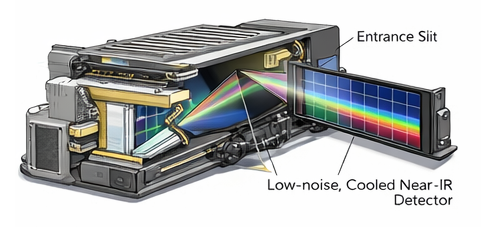
\includegraphics[width=0.85\linewidth,height=0.42\textheight,keepaspectratio]{book_media/image4.png}
\end{figure}

Fig. 4. Conceptual illustration of the spectroscopic instrument(AI)

The spectroscopic instrument suite is designed to provide continuous wavelength coverage across the optical and near-infrared regimes, with an emphasis on high-precision spectroscopy at low- to moderate-spectral resolution. These instruments support the physical characterization of astronomical sources required for time-domain astronomy, compact-object studies, and galaxy evolution research.

The design minimizes the number of moving components in order to maximize reliability and calibration consistency while ensuring long-term stability for time-series spectroscopic observations. The spectrographs incorporate optical assemblies, dispersive elements, and low-noise near-infrared detectors, with particular attention given to thermal and mechanical stability so that performance variations remain minimal throughout extended mission operations.

A comprehensive internal calibration system is incorporated to support high-precision spectrophotometric measurements. This capability reduces dependence on calibration observations of external astronomical standards, improves calibration repeatability, and enhances overall observing efficiency. By maintaining a stable and well-characterized instrumental response over long timescales, the spectroscopic instruments provide the precision required for a broad range of astrophysical investigations, including transient phenomena, exoplanet atmosphere studies, compact-object physics, and galaxy evolution.

\section{Optional High-Contrast Observing Capability and Future Expandability}\label{optional-high-contrast-observing-capability-and-future-expandability}

Direct imaging of exoplanets and high-contrast observations are recognized as among the most scientifically impactful areas of future space astronomy. In particular, high-contrast observing techniques, including coronagraphy, are essential for directly separating and detecting faint planetary signals around bright host stars. However, such observations impose extremely stringent requirements on wavefront stability, thermal stability, and long-term pointing stability across the entire telescope optical system.

The baseline mission configuration of the 3.5-meter Segmented-Mirror Robotic Space Telescope is optimized for time-domain and multi-messenger astronomy as well as precision time-series observations. A dedicated coronagraph for exoplanet direct imaging is therefore not defined as a mandatory instrument in the initial mission configuration. This reflects the mission's practical design philosophy, which emphasizes strict control of schedule, cost, and technical risk.

Nevertheless, the optical design and overall observatory architecture are being examined in a manner that does not preclude the future addition or upgrade of high-contrast observing capabilities. In other words, the mission intentionally preserves design flexibility for the possible integration of an optional high-contrast module within the optical path, the expansion of wavefront sensing and control capabilities, and the adaptation of observing and operations software for future high-contrast observing modes.

This approach ensures that the mission is not limited solely to its near-term scientific objectives. Instead, it enables the telescope to serve as a technological and operational precursor for future direct-imaging missions targeting exoplanets, including flagship-class space observatories that may search for potentially habitable worlds in the coming decades. Thus, even if the 3.5-meter space telescope performs high-contrast observations only in a limited capacity during its early phase, it can be defined as an observatory whose role may expand progressively through international collaboration and improvements in technology readiness.

In summary, the mission does not impose an exoplanet coronagraph as a core requirement of the initial science payload, while strategically preserving the architectural flexibility needed to accommodate future expansion toward high-contrast observations. This represents a balanced design choice that manages mission risk without prematurely closing off future scientific opportunities.

\begin{figure}[htbp]\centering
  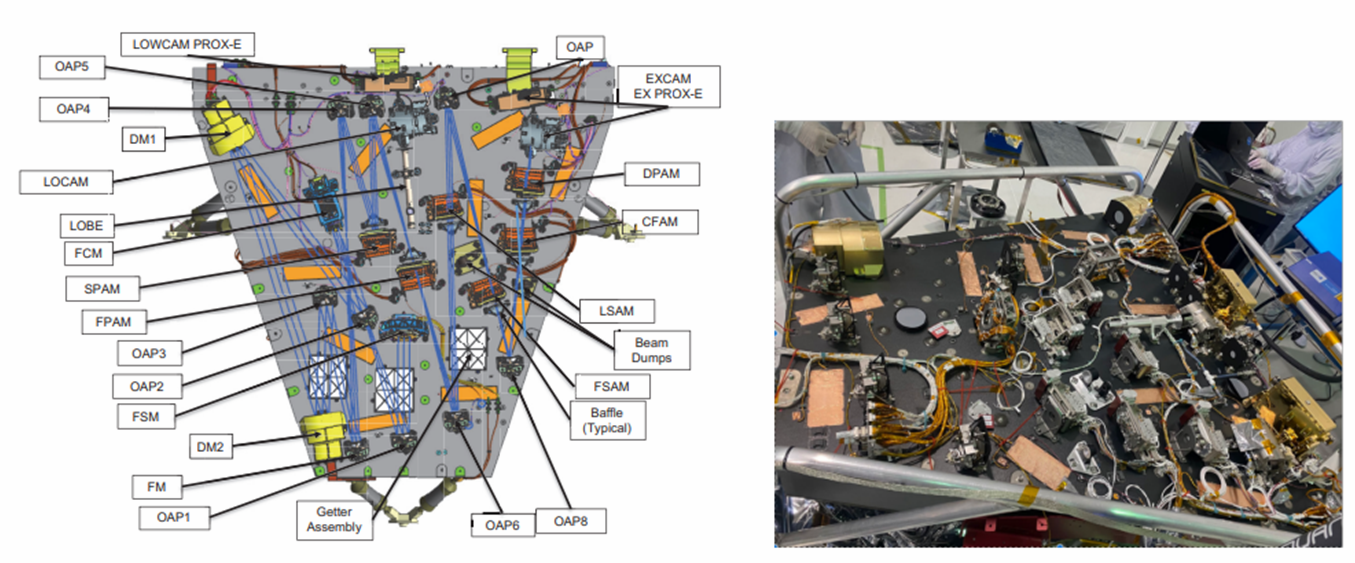
\includegraphics[width=0.85\linewidth,height=0.42\textheight,keepaspectratio]{book_media/image5.png}
\end{figure}

Fig. 5. Exoplanet coronagraph of the Nancy Grace Roman Space Telescope (Vanessa et al. 2023)

\section{Summary of Design Performance and Expandability}\label{summary-of-design-performance-and-expandability}

The 3.5-meter Segmented-Mirror Robotic Space Telescope is designed as a space observatory that combines near-diffraction-limited image quality in the optical and near-infrared wavelength ranges, highly stable pointing performance, and rapid-response observational capability. These capabilities are not represented by a single performance metric; rather, they are achieved as a system-level outcome through the integrated operation of the optical system, attitude control system, thermal control architecture, and mission operations concept.

The design is intended not only to satisfy the initial mission requirements but also to intentionally preserve flexibility for future instrument upgrades and the expansion of operational strategies. This design choice ensures that the observatory will not be limited to short-term scientific achievements, but will instead function as a core infrastructure for Korean space astronomy over the long term.

\chapter{Scientific Objectives}
\section{Cosmology}\label{cosmology}

\subsection{Cosmic Acceleration, Dark Energy, and Dark Matter}\label{cosmic-acceleration-dark-energy-and-dark-matter}

The accelerated expansion of the Universe was first discovered in 1998 through observations of Type Ia supernovae and has since been strongly confirmed by a wide range of cosmological observations [8,9]. This discovery became a foundation of the standard ΛCDM cosmological model and led to the interpretation that dark energy accounts for approximately 70\% of the total energy density of the Universe. However, the physical nature of dark energy---whether it is truly the cosmological constant Λ or a dynamical field that evolves with time---remains one of the central questions at the frontier of modern cosmology.

The 3.5-meter-class multiwavelength space telescope is designed to address this problem in a manner distinct from all-sky survey missions that maximize statistical coverage. Instead, it will reduce systematic uncertainties in cosmological parameters and enhance physical interpretability through high-resolution, high-precision deep observations. Rather than performing shallow observations over the widest possible area, the telescope will repeatedly survey homogeneous deep fields covering several hundred square degrees, enabling precision tests of both the properties of dark energy and the validity of gravitational theory.

The key observables describing cosmic acceleration are the distance--redshift relation and the cosmic expansion rate, H(z). These quantities can be measured directly through the Hubble diagram constructed using Type Ia supernovae as standard candles. By simultaneously utilizing a broad wavelength range from 0.2 to 3.0 μm, the telescope will enable supernova color corrections and evolutionary corrections to be performed within a single, internally consistent framework. This capability removes major limitations of ground-based observations, including variations in atmospheric transmission and wavelength-dependent calibration uncertainties, and enables stable photometric measurements with precision better than 0.01 mag.

As a result, a sample of several thousand high-redshift supernovae, extending to approximately z ≈ 1.5, could constrain the present-day value of the dark energy equation-of-state parameter, w₀, and its time-evolution parameter, wₐ, to approximately ±0.05 and ±0.2, respectively. Beyond improving statistical precision, such a dataset would provide a practical means of testing the temporal evolution of dark energy by directly controlling systematic uncertainties associated with color correction and dust extinction.

Another independent probe of cosmic acceleration is provided by Baryon Acoustic Oscillations (BAOs). Acoustic waves that propagated through the primordial plasma of the early Universe have left an imprint on the large-scale distribution of galaxies as a characteristic length scale of approximately 150 Mpc. This standard ruler enables simultaneous measurements of the angular diameter distance, (D\_A(z)), and the Hubble parameter, (H(z)). The 3.5-meter telescope will conduct spectroscopic observations of emission-line galaxies in the intermediate-redshift range ((z \textbackslash approx 0.5)--2.5) at spectral resolutions of (R \textbackslash approx 500)--1000, enabling the construction of photometric--spectroscopic redshift samples containing millions of galaxies. Although the mission is not intended to perform an ultra-wide all-sky survey, its strategy of deep and homogeneous observations over selected fields provides a valuable independent benchmark for cross-validating the statistical results obtained by missions such as Euclid and the Roman Space Telescope. In particular, when combined with Type Ia supernova distance measurements obtained in the same fields, these observations enable direct tests of the consistency of geometric distance indicators, providing a powerful means of distinguishing among competing dark-energy models.

However, it remains unclear whether cosmic acceleration is driven by a new energy component, namely dark energy, or by a modification of gravity on cosmological scales. Discriminating between these possibilities requires measurements not only of the expansion history of the Universe but also of the growth rate of cosmic structure. Weak gravitational lensing, commonly referred to as cosmic shear, is one of the most powerful observational tools for directly probing the growth of structure.

The proposed telescope will deliver diffraction-limited angular resolution of approximately 0.21 arcseconds at 3 μm, together with a highly stable point-spread function (PSF) over time. These characteristics enable precise measurements of subtle distortions in galaxy shapes induced by weak gravitational lensing. Through deep observations covering several hundred square degrees, the mission is expected to achieve a galaxy shape density of approximately 30--40 galaxies per square arcminute, allowing precise determinations of key cosmological parameters, including (\textbackslash sigma\_8), (\textbackslash Omega\_m), and the growth-rate parameter (f\textbackslash sigma\_8(z)).

These quantities describe how rapidly cosmic structures grow over time and provide direct observational tests capable of distinguishing the standard ΛCDM framework from modified-gravity theories such as (f(R)) gravity and the Dvali--Gabadadze--Porrati (DGP) model. In this sense, the telescope serves not merely as an instrument for measuring how fast the Universe is expanding, but as an experimental facility for investigating how gravity itself operates on the largest scales in the Universe.

Dark matter research is closely linked to these precision cosmological observations. Weak-lensing mass maps enable the direct reconstruction of the three-dimensional distribution of dark matter, while the evolution of the galaxy cluster mass function provides strong constraints on theories of structure formation. In particular, measurements of substructure and time delays in strong gravitational lens systems allow the subhalo mass function to be inferred from the detailed morphology of Einstein rings and the flux ratios of multiple images. These observations provide critical information for determining whether dark matter is cold and effectively collisionless, or whether it exhibits small-scale suppression characteristic of alternative models such as warm dark matter or fuzzy dark matter.

Furthermore, measurements of offsets among the distributions of gas, stars, and dark matter in merging galaxy clusters can place stringent upper limits on the self-interaction cross section of self-interacting dark matter (SIDM). Such observations are essential for probing the macroscopic properties of dark matter through astrophysical means, complementing particle-physics experiments that are often insensitive to these large-scale phenomena.

Ultimately, the cosmology program of the 3.5-meter space telescope does not rely on any single observational technique. Type Ia supernovae and BAO measurements probe the geometric expansion history of the Universe, while weak and strong gravitational lensing constrain the growth of cosmic structure and the distribution of dark matter. By combining these complementary approaches, it becomes possible to distinguish, at the 3--5σ level, whether cosmic acceleration is driven by a simple cosmological constant (Λ), a dynamically evolving form of dark energy, or a modification of gravity itself.

In addition, independent distance-ladder measurements and time-delay lensing observations can provide complementary constraints on the Hubble constant, offering a potential avenue for resolving the currently observed Hubble tension ((H\_0) tension). These measurements are particularly valuable because they rely on fundamentally different physical principles and systematic uncertainties than traditional cosmological probes.

In summary, this telescope is not designed primarily to expand all-sky survey statistics. Rather, it functions as a precision cosmology laboratory capable of physically discriminating among competing cosmological models and calibrating the systematic uncertainties that limit current large-scale survey missions. The temporal evolution of dark energy, the validity of gravitational theory on cosmological scales, and the macroscopic properties of dark matter will be directly constrained by the mission\textquotesingle s key observations. The resulting datasets are expected to provide foundational evidence that will shape the direction of cosmological theory and fundamental physics for decades to come.

\subsection{Unveiling the Nature of Dark Matter}\label{unveiling-the-nature-of-dark-matter}

Dark matter represents one of the most fundamental challenges at the intersection of cosmology and particle physics. Unlike ordinary matter, dark matter interacts only weakly, if at all, through electromagnetic forces, making it effectively invisible to direct observation. Nevertheless, its existence has been established with a high degree of confidence through a wide range of astrophysical observations, including galaxy rotation curves, the internal dynamics of galaxy clusters, gravitational lensing phenomena, and anisotropies in the Cosmic Microwave Background (CMB) [15]. These indirect lines of evidence indicate that dark matter constitutes more than five times the mass of ordinary baryonic matter and serves as the gravitational framework upon which galaxies and large-scale cosmic structures are formed.

The standard ΛCDM (Lambda Cold Dark Matter) model assumes that dark matter consists of cold, collisionless particles. This framework successfully explains the formation of large-scale structure, the observed properties of galaxy rotation curves, and the detailed features of the CMB with remarkable accuracy. Despite its observational success, however, the fundamental particle nature of dark matter remains unknown, and no viable dark matter candidate has yet been conclusively detected [16].

Determining the true nature of dark matter requires a comprehensive approach that combines astrophysical observations, particle-physics experiments, and cosmological datasets. Only through the integration of these complementary avenues of investigation can the physical properties of dark matter be constrained and its role in the evolution of the Universe be fully understood.

\textbf{Dark Matter Candidates and Theoretical Frameworks}

Because dark matter cannot be explained by any particle contained within the Standard Model of particle physics, a wide variety of theoretical scenarios introducing new particles and interactions have been proposed. The oldest and most extensively studied candidates are Weakly Interacting Massive Particles (WIMPs), which are modeled as electrically neutral particles that interact predominantly through gravity and only very weakly through other fundamental forces. Other prominent candidates include axions, sterile neutrinos, and ultralight bosonic particles that may form Bose--Einstein condensate-like states. These candidates give rise to distinct formation histories and structure-formation mechanisms, leading to observable differences in astrophysical and cosmological phenomena [17].

From a theoretical perspective, dark matter candidates are commonly classified according to their production mechanisms and thermodynamic evolution in the early Universe. Particles that were initially in thermal equilibrium and later decoupled through a freeze-out process can naturally account for the present-day relic density of dark matter. The resulting abundance depends sensitively on the particle mass, interaction cross section, and the expansion history of the Universe. In addition to these thermal production scenarios, contemporary dark matter research increasingly considers non-thermal production mechanisms and models involving complex dark sectors with multiple particle species and interactions. Such frameworks provide a rich theoretical landscape that extends well beyond the traditional WIMP paradigm and may offer explanations for observational phenomena that are difficult to reconcile within the standard cold dark matter model.

\textbf{Observational Constraints and Experimental Searches}

Although astrophysical observations provide compelling evidence for the existence of dark matter, they do not directly reveal its microscopic physical properties. Galaxy rotation curves indicate that dark matter forms extended halos surrounding galaxies, a prediction that is broadly consistent with the ΛCDM framework. On larger scales, gravitational lensing and X-ray observations of galaxy clusters enable the reconstruction of their mass distributions, providing quantitative measurements of the spatial distribution of dark matter.

Experimental searches for dark matter can be broadly divided into three categories. First, direct detection experiments seek signals produced when dark matter particles scatter off atomic nuclei in highly sensitive terrestrial detectors. Second, indirect detection searches attempt to observe products of dark matter annihilation or decay, such as gamma rays, electrons, positrons, or other high-energy particles. Third, collider searches investigate signatures of dark matter production in high-energy particle collisions, typically through measurements of missing energy and momentum. While none of these approaches has yet produced definitive evidence for a dark matter particle, experimental sensitivities continue to improve steadily, placing increasingly stringent constraints on theoretical models [18].

\textbf{Cosmological Data and Sensitivity to Structure Formation}

Numerical simulations of cosmic structure formation demonstrate that the properties of large-scale structure are highly sensitive to the free-streaming length of dark matter particles. For example, hot dark matter, characterized by relativistic particle velocities in the early Universe, suppresses the formation of small-scale structures. In contrast, cold dark matter promotes structure formation even on relatively small scales, allowing galaxies and substructures to emerge efficiently. These differences are reflected in observable properties of the cosmic web, including the distribution of galaxies, filamentary structures, and the abundance of dwarf galaxies.

Recent studies have also explored the possibility of weak interactions between dark matter and neutrinos, challenging the traditional assumption that dark matter is entirely non-interacting apart from gravity. Such interactions could leave detectable imprints on cosmic structure formation and the evolution of density fluctuations. In addition, gravitational lensing observations have begun to reveal evidence for small-scale dark matter clumps within and around galaxies, providing new datasets that can be directly compared with the predictions of the ΛCDM model and its alternatives.

Together, these observational and theoretical developments highlight the growing importance of combining cosmological observations, astrophysical measurements, and particle-physics experiments to uncover the fundamental nature of dark matter and its role in shaping the evolution of the Universe.

\textbf{Future Prospects and Cosmological Experiments}

Deep and high-precision cosmological observatories, such as a 3.5-meter space telescope, have the potential to probe the fine structure and dynamical properties of dark matter with unprecedented accuracy. For example, by analyzing weak and strong gravitational lensing distortions, it is possible to reconstruct the three-dimensional structure of dark matter halos and thereby place indirect constraints on the interaction properties predicted by particle physics models. When combined with ground-based experiments, these cosmological approaches will play a crucial role in unveiling the true nature of dark matter.

\subsection{Initial Conditions of the Universe and Their Empirical Tests}\label{initial-conditions-of-the-universe-and-their-empirical-tests}

The initial conditions of the Universe and their empirical verification constitute one of the central challenges in cosmology. Our understanding of the formation and evolution of cosmic structures originates from these primordial conditions. The early Universe existed in an extremely hot and dense state and subsequently evolved through rapid expansion and cooling, eventually giving rise to the large-scale structures observed today. The initial conditions are primarily tested through comparisons between theoretical predictions and observations of the anisotropies in the Cosmic Microwave Background (CMB), the distribution of large-scale structures, and primordial nucleosynthesis. These observational tests form the foundation of the ΛCDM cosmological model and play a crucial role in characterizing the physics of the early Universe [19].

The standard paradigm of modern cosmology assumes that the initial conditions of the Universe originated from density fluctuations described by a random Gaussian field. These fluctuations are believed to have been generated during the inflationary epoch, a process in which microscopic quantum fluctuations were amplified into macroscopic density perturbations spanning cosmological scales. Inflation not only provides a mechanism for generating the primordial fluctuations that seed cosmic structure formation but also offers elegant solutions to the horizon, flatness, and homogeneity problems. Consequently, it has become the leading theoretical framework for explaining the initial conditions imprinted in both the CMB and the large-scale structure of the Universe [20]. The statistical properties of these primordial fluctuations and their subsequent evolution are preserved as precise patterns in the temperature and polarization anisotropies of the CMB.

CMB observations are often regarded as a direct snapshot of the initial conditions of the Universe. In particular, the \textbf{Planck} satellite provided highly precise measurements of temperature and polarization anisotropies, enabling stringent constraints on the spectrum and statistical properties of primordial fluctuations [10]. The Planck data show excellent agreement with the predictions of the ΛCDM model, indicating that the primordial perturbations are well described by an almost random Gaussian distribution and exhibit near scale invariance. Specifically, the scalar spectral index, $n_s$, is found to be close to unity, while any detectable level of non-Gaussianity remains extremely small within current observational limits. These results provide important clues for reconstructing the underlying field dynamics that established the initial conditions of the Universe [10].

Another key avenue for testing the initial conditions is the evolution of large-scale structure. Cosmic structures originated from primordial density fluctuations and subsequently grew under the combined effects of cosmic expansion and gravitational instability, eventually forming the galaxies, galaxy clusters, and vast filamentary structures observed today [21]. This growth process can be modeled through numerical simulations and compared with observed galaxy distributions, allowing the initial conditions and evolutionary mechanisms to be tested in a unified framework. In particular, the amplitudes and correlations of fluctuations present in the primordial density field are transformed through gravitational interactions and are reflected in the present-day two-point correlation function of matter. Consequently, the statistical properties of the observed matter distribution provide an additional and independent window for testing primordial fluctuations [22,23].

Primordial nucleosynthesis provides another powerful probe of the early Universe by predicting the relative abundances of hydrogen, helium, and lithium. These predictions are highly sensitive to the density, temperature, and baryon content of the Universe during its earliest stages [24]. Observations of elemental abundances are generally consistent with theoretical expectations, enabling constraints to be placed on the thermodynamic conditions and expansion rate of the early Universe. In particular, primordial nucleosynthesis offers an important and independent determination of the baryon density, complementing constraints derived from CMB observations.

Taken together, CMB anisotropies, the large-scale distribution of matter, and primordial nucleosynthesis provide complementary tests of the initial conditions of the Universe. For example, the CMB directly measures the primordial fluctuation spectrum, whereas large-scale structure observations reveal how that spectrum evolved over cosmic time. By combining these observational probes, cosmologists can determine the initial conditions and cosmological parameters with significantly greater precision than would be possible using any single dataset alone [25,26]. Such joint analyses enable high-confidence tests of cosmological models that cannot be achieved through individual observational probes in isolation.

Another important prediction of inflationary theory is the possible existence of \textbf{non-Gaussianity} in the primordial fluctuations. While the majority of primordial perturbations are expected to follow a Gaussian distribution, many inflationary models predict small but measurable deviations from Gaussianity [27]. Precision analyses of CMB and large-scale structure data place increasingly stringent constraints on such non-Gaussian signatures, providing a powerful means of distinguishing among competing classes of inflationary models [10,19,28]. Measurements of the level of non-Gaussianity therefore offer direct insights into the interactions and dynamics of the fields that governed the early Universe.

The verification of primordial conditions has also benefited significantly from measurements of the polarization of the Cosmic Microwave Background. In particular, \textbf{B-mode polarization} provides a potential direct probe of the primordial gravitational-wave background, which is predicted to have been generated during the earliest stages of inflation [29]. Although the detection of a primordial B-mode signal remains challenging because of contamination from Galactic dust emission, future CMB polarization experiments and high-precision space-based observatories are expected to improve the separation of foreground signals and enhance the prospects for a definitive detection.

Precision cosmological observatories such as the proposed telescope can further advance studies of the early Universe by directly probing the epoch of reionization and the formation of the first cosmic structures after the CMB era. For example, observations of the distribution of galaxies and galaxy clusters at intermediate to high redshifts, combined with measurements of the neutral hydrogen 21-cm line, can provide a deeper and more comprehensive window into the initial conditions of the Universe and their subsequent evolution [30,31]. Such observations extend beyond simply testing the expansion history or the growth of density fluctuations; they form part of a \textbf{multimodal observational strategy} aimed at uncovering the fundamental physics of the early Universe through multiple complementary probes.

\section{Galaxies}\label{galaxies}

\subsection{Cosmic Reionization, Large-Scale Structure, and Cosmological Probes}\label{cosmic-reionization-large-scale-structure-and-cosmological-probes}

The \textbf{Epoch of Reionization (EoR)} refers to the period in cosmic history following the era when the Universe remained largely neutral (z≳6z \textbackslash gtrsim 6z≳6), during which ultraviolet radiation emitted by the first generations of stars and galaxies reionized the hydrogen in the intergalactic medium (IGM). This epoch had profound consequences for the formation of large-scale cosmic structures and the evolution of the free-electron density in the Universe. It also serves as a critical astrophysical background for interpreting cosmological observables such as the matter distribution, gravitational lensing signals, and secondary anisotropies of the Cosmic Microwave Background (CMB). Understanding the processes of reionization and the associated formation of cosmic structures is therefore one of the fundamental challenges of modern cosmology [32].

Reionization is the outcome of a highly complex interplay of astrophysical processes. Star formation within galaxies, subsequent supernova explosions, feedback from active galactic nuclei (AGN), and the influence of cosmic rays all affect the escape fraction of ionizing ultraviolet photons and the thermal and dynamical state of the surrounding medium. Recent studies have demonstrated through numerical simulations that internal galactic feedback processes influence not only the evolution of the EoR itself but also the overall distribution of matter in the Universe. For example, galaxy-formation feedback can suppress star formation efficiency, thereby modifying both the timing and the amplitude of reionization. These effects, in turn, alter the interpretation of cosmological observables derived from large-scale surveys and precision cosmological measurements [33].

The state of cosmic reionization in the early Universe is reflected in several key cosmological observables. In particular, the post-reionization scattering signature imprinted on the Cosmic Microwave Background (CMB), including its E-mode polarization and temperature anisotropy patterns, is closely linked to the cumulative evolution of the free-electron density over cosmic time. High-redshift objects, such as distant quasars and Lyman-α emitting galaxies, provide valuable observational windows into the inhomogeneous transition from a neutral to an ionized Universe [35].

Cosmic reionization and the formation of large-scale structure (LSS) are intimately connected. Structures originating from primordial density fluctuations grow through gravitational instability, eventually forming the vast cosmic web of filaments, galaxy clusters, and superclusters observed today. This process not only constrains cosmological parameters---such as the matter density parameter (Ωm\textbackslash Omega\_mΩm), characteristic clustering scales, and the nature of gravity---but also leaves observable imprints from reionization. In particular, the size and distribution of ionized regions generated during reionization influence various LSS observables, including the matter power spectrum and galaxy environments. Reionization can suppress baryonic clustering on small scales, thereby modifying the evolution of cosmic structures [36].

More specifically, feedback mechanisms---including active galactic nucleus (AGN) outflows, supernova explosions, and cosmic-ray pressure---can redistribute baryonic matter beyond the boundaries of their host dark matter halos. Compared with models that consider only gravitational evolution, these processes suppress power on small scales in the matter power spectrum. Such suppression can introduce systematic biases when interpreting precision measurements of large-scale structure in combination with CMB observations, including weak gravitational lensing (cosmic shear) as well as the kinetic and thermal Sunyaev--Zel'dovich (kSZ and tSZ) effects [36].

Reionization itself is governed not only by internal galactic processes but also by local environmental conditions, such as proximity to massive galaxy clusters and the distribution of collapsed dark matter halos. These factors determine important characteristics of the reionization process, including the sizes of ionized bubbles and the spatial inhomogeneity of ionization fronts. Such inhomogeneities can be directly probed through observations of the Lyman-α forest and the neutral hydrogen 21-cm line, providing a means of simultaneously tracing both cosmic structure formation and the physical mechanisms driving the Epoch of Reionization [35].

Within this framework, the estimation of cosmological parameters---such as the Hubble constant, the matter and dark energy densities, and the scalar spectral index ($n_s$)---cannot rely solely on observational data. Variations in the matter distribution induced by galaxy feedback processes and reionization can significantly distort cosmological signals. Consequently, modern cosmology increasingly emphasizes the systematic modeling of the interplay between reionization and large-scale structure formation. Hydrodynamical simulations and halo-based modeling have become essential tools in this effort. By jointly accounting for feedback strength, halo mass functions, and the relationship between galaxy mass and environment, these simulations enable quantitative assessments of how reionization influences observable matter distributions and cosmological signals [35].

For example, measurements of the \textbf{kinetic Sunyaev--Zel'dovich (kSZ) effect} probe the distribution and motion of free electrons after the Epoch of Reionization. Because the free-electron density field exhibits significant spatial asymmetries associated with cosmic structures, the resulting kSZ signal can produce deviations from the matter power spectrum predicted by the standard ΛCDM model. These discrepancies can be mitigated through more accurate modeling of baryonic processes, such as AGN feedback, which strongly influence halo evolution and the redistribution of baryonic matter.

Ultimately, a variety of physical processes occurring within galaxies---including supernova feedback, AGN-driven winds, and ionizing radiation associated with reionization---play central roles in shaping the reionization history of the Universe. The consequences of these processes are imprinted on large-scale structure and a wide range of cosmological observables. As a result, studies of reionization and large-scale structure have evolved beyond a purely astrophysical problem and now constitute an integrated observational and theoretical framework for constraining cosmological parameters and testing the initial conditions of the Universe.

\section{Compact Objects}

\subsection{Investigating White Dwarf Internal Matter Properties with a 3.5 m Space Telescope}

White dwarfs are the dense stellar remnants left behind after stars with masses comparable to that of the Sun complete their evolutionary lifecycles. Their interiors are supported by electron degeneracy pressure, representing an extreme state of matter that cannot be reproduced under terrestrial laboratory conditions. These environments contain highly compressed plasma and provide a unique laboratory for studying fundamental physics at the intersection of cosmology, particle physics, and astrophysics.

Most white dwarfs possess cores composed primarily of carbon (C) and oxygen (O), although more massive progenitors may produce oxygen--neon (O--Ne) cores in extreme cases. The core composition is closely linked to the nuclear-burning history of the progenitor star. In particular, the carbon-to-oxygen ratio and the detailed distribution of chemical elements depend strongly on the star's initial mass and the rates of nuclear reactions that occurred during its evolution. These properties subsequently influence the cooling timescale of the white dwarf, the progression of crystallization within its interior, and various aspects of its surface and atmospheric physics [36].

One of the most powerful tools for investigating the internal properties of white dwarfs is asteroseismology. Pulsating white dwarfs exhibit non-radial oscillation modes generated within their interiors, and the frequencies of these oscillations are highly sensitive to the internal density structure, chemical stratification, and temperature distribution. By comparing observed pulsation periods and mode characteristics with theoretical models, it is possible to place quantitative constraints on core composition, the state of degenerate electrons, thermal conductivity, and other fundamental physical properties of the stellar interior. For example, the comprehensive review by Córsico (2019) [37] describes how different pulsation modes effectively ``scan'' the deep interior of a white dwarf, providing estimates of quantities such as the stellar mass, rotation rate, and magnetic-field strength.

Studies of white dwarf interiors are closely connected to their core composition and cooling history. After nuclear fusion ceases, a white dwarf gradually cools by radiating away its residual thermal energy over timescales of billions of years. The cooling process is governed by the interplay between conductive energy transport through degenerate electrons and radiative energy loss from the stellar surface. Temperature gradients between the core and the surface, together with diffusion and convection at compositional boundaries, influence both the cooling rate and the observed pulsation modes. Detailed analyses of pulsation signals therefore make it possible to constrain the equation of state of matter in the stellar interior---information that cannot be obtained through measurements of luminosity and temperature alone [38].

A 3.5 m space telescope would provide significant advantages for studying the internal properties of white dwarfs in at least three major ways.

First, it would enable high-precision analyses of pulsation modes through photometric and spectroscopic observations. The pulsation periods of white dwarfs, typically on the order of several hundred seconds, are closely linked to atmospheric properties, core composition, and the state of electron degeneracy pressure. Equipped with highly sensitive instruments, a space telescope can obtain uninterrupted light curves free from atmospheric distortions, allowing the phases and amplitudes of pulsation modes to be measured with exceptional precision. Data from missions such as Gaia and Kepler have already revolutionized the field of white dwarf asteroseismology. A next-generation space telescope would be capable of detecting even subtler oscillation signals, thereby enabling the reconstruction of increasingly detailed information about the internal structure of white dwarfs [39].

Second, a 3.5 m space telescope would enable detailed studies of compositional stratification and the mean atomic weight of white dwarf cores. Such investigations can be carried out not only through pulsation-mode analysis but also through spectroscopic chemical signatures. Most observed white dwarfs possess atmospheres dominated by either hydrogen (H) or helium (He), while some exhibit surface metal pollution resulting from the accretion of external material. These metal-contaminated surface layers provide important clues about the presence and distribution of heavier elements within the stellar interior and can help constrain the evolutionary history of the white dwarf [39].

Third, the telescope would provide a unique opportunity to test crystallization processes and the equation of state of degenerate matter. White dwarf interiors reach extremely high densities, typically on the order of 10610\^{}6106--107~g cm−310\^{}7\textbackslash{} \textbackslash mathrm\{g\textbackslash,cm\^{}\{-3\}\}107~gcm−3. Under such conditions, matter can undergo a phase transition from a plasma state to a crystalline state on a macroscopic scale. This crystallization process releases latent heat and produces a measurable cooling delay, an effect that has already been observed in some high-mass white dwarfs. The energy released during crystallization leaves characteristic signatures in the white dwarf luminosity function. Through long-term monitoring and statistical sampling, a space telescope can quantitatively measure these signatures and provide direct empirical tests of dense-matter physics.

The study of white dwarf interior properties also has important cosmological implications. For example, the use of Type Ia supernovae as standard candles is closely linked to the pre-explosion structure of white dwarf progenitors. Internal composition, chemical stratification, and the degree of electron degeneracy can influence the luminosity and color corrections applied to Type Ia supernova observations, thereby contributing to systematic uncertainties in cosmological distance measurements. Consequently, precise studies of white dwarf interiors improve not only our understanding of white dwarf physics but also the accuracy of cosmological parameter determinations derived from Type Ia supernova surveys.

In conclusion, a 3.5 m space telescope would make a unique and transformative contribution to the study of white dwarf interior matter. Its ability to perform uninterrupted long-duration observations free from atmospheric interference, combined with high-sensitivity spectroscopic capabilities and broad wavelength coverage, would significantly strengthen observational constraints on compositional stratification, the equation of state of degenerate matter, and the cooling and crystallization processes occurring within white dwarfs. These data would enhance our understanding of white dwarf physics while also supporting a wide range of cosmological applications, including the calibration of Type Ia supernova standard candles and the reconstruction of the star-formation and evolutionary history of galaxies.

\subsection{Analyzing Circumstellar Material Around High-Density Compact Objects}\label{analyzing-circumstellar-material-around-high-density-compact-objects}

The distribution and physical properties of circumstellar material around high-density compact objects, particularly white dwarfs, preserve valuable records of planetary systems that survived the final stages of stellar evolution. Because white dwarfs possess extremely strong gravitational fields, the detection of metal accretion onto their surfaces indicates the presence of material that remains in stable orbit around the star. This material is generally believed to originate from remnant planetary systems, such as asteroid belts, minor planets, or disrupted planetary bodies that survived the host star's evolution [41,42].

A primary driver of circumstellar material around white dwarfs is planetary debris. Following stellar evolution, surviving asteroids or planetary remnants may be perturbed onto highly eccentric orbits that bring them close to the white dwarf's Roche limit. Once inside this critical distance, tidal forces can disrupt these bodies, fragmenting them into smaller particles and gas. The resulting debris is redistributed into a circumstellar debris disk surrounding the central star [42]. Such disks are frequently detected through infrared excess emission and provide strong evidence for the long-term presence of circumstellar material around white dwarfs [40].

\begin{figure}[htbp]\centering
  
\includegraphics[width=0.85\linewidth,height=0.42\textheight,keepaspectratio]{book_media/image6.jpeg}
\end{figure}

Fig. 6. White dwarf(AI)

The detection of heavy elements such as calcium (Ca), magnesium (Mg), and iron (Fe) in white dwarf atmospheres is commonly referred to as metal pollution\textbf{.} This phenomenon is particularly significant because the strong gravitational fields of white dwarfs should cause heavy elements to settle out of the atmosphere on relatively short timescales. The continued presence of these metals therefore implies ongoing replenishment by external material [40,43]. In other words, material from the surrounding debris disk is continuously accreted onto the white dwarf surface. Measurements of the atmospheric abundances of these elements provide a unique opportunity to infer the composition and distribution of the disrupted planetary material from which they originated.

Collisions and tidal disruption are considered the principal mechanisms responsible for disk formation and material redistribution. For example, observations of the system WD 1145+017 have revealed the ongoing disintegration of small planetary bodies in close proximity to a white dwarf [44]. These events are observed as irregular transit dimming signatures caused by clouds of dust and debris passing in front of the star. In addition, interactions among dust particles and gaseous material within the disk play a critical role in determining the dynamical evolution of the system. Several systems observed with the Spitzer Space Telescope have exhibited variations in disk brightness and color that are associated with changes in particle-size distributions, demonstrating the importance of disk dynamics and matter interactions within circumstellar debris environments [46].

\textbf{Material Distribution and Composition Analysis}

The chemical composition of circumstellar material around white dwarfs provides important clues about the nature of its parent bodies. A study by Xu et al. [47], based on an analysis of 19 white dwarf systems, found that the chemical abundances of the surrounding material exhibit patterns similar to those of terrestrial planets in the Solar System, with relatively consistent ratios of iron (Fe), magnesium (Mg), and calcium (Ca). These results suggest that the material surrounding white dwarfs is predominantly composed of rocky, terrestrial-like matter. Such analyses are derived from high-resolution spectroscopic observations and are inferred from the relative abundances of metallic elements detected in white dwarf atmospheres. By comparing these atmospheric abundances with models of diffusion and accretion, it is possible to reconstruct the composition of the disrupted planetary material from which they originated.

\textbf{Mass Accretion and Condensation Processes}

Theoretical studies of the mechanisms by which circumstellar material is transported onto white dwarf surfaces are closely linked to the Poynting--Robertson (PR) drag effect. Rafikov [48] demonstrated through numerical modeling that PR drag causes disk particles to gradually lose angular momentum and spiral inward toward the white dwarf. During this inward migration, dust particles may undergo sublimation, transforming into gaseous material that can ultimately accrete onto the stellar surface. This process provides a natural pathway for the continuous replenishment of metals observed in polluted white dwarf atmospheres.

Subsequent studies have expanded upon this framework by examining the coupled evolution of gas and dust within circumstellar disks. These investigations have proposed mechanisms involving gas--particle interactions, enhanced inward acceleration, and runaway accretion, which can lead to unstable mass-transfer episodes and significantly elevated accretion rates [48]. Such processes are believed to play a key role in shaping the dynamical evolution of debris disks and in regulating the flow of planetary material onto white dwarfs. Understanding these accretion mechanisms is therefore essential for interpreting the observed properties of polluted white dwarfs and for reconstructing the long-term evolution of remnant planetary systems.

\textbf{Disk Structure and Overall Dynamics}

Observationally, circumstellar disks around white dwarfs consist of gaseous material and dusty debris and are most commonly detected through their infrared excess (IR excess) emission. Well-known examples include the white dwarfs G29-38 and GD 362. In particular, infrared observations of G29-38 with the Spitzer Space Telescope revealed that a significant fraction of the dust particles is concentrated near the white dwarf's Roche radius. This system has become one of the canonical examples for understanding the processes of disk formation and the redistribution of tidally disrupted planetary material into a circumstellar disk.

Furthermore, the observed correlation between the degree of metal pollution and the presence of circumstellar disks provides quantitative information on accretion rates and the distribution of surrounding material. Interestingly, some white dwarfs exhibit clear atmospheric metal pollution despite showing no detectable debris disk. This suggests the existence of tenuous or low-mass debris populations that remain below current observational detection limits [49]. Such cases highlight the continuing importance of improving observational sensitivity and refining models of particle-size distributions in studies of circumstellar material around white dwarfs.

\textbf{Significance of Observations with a Space Telescope}

A 3.5 m-class space telescope, equipped with high-resolution spectroscopic capabilities and enhanced infrared sensitivity, would provide unprecedented opportunities to investigate the structure, composition, and dynamical evolution of circumstellar material around white dwarfs. In particular, infrared spectroscopy and particle-size distribution measurements that were only possible for limited samples with missions such as the James Webb Space Telescope and the Spitzer Space Telescope could be extended to a much larger and more diverse population of systems. Such observations would enable detailed studies of the formation, evolution, and disruption of debris disks over both spatial and temporal scales, while also allowing quantitative assessments of how circumstellar material influences white dwarf evolution and the long-term development of planetary systems.

\section{Conclusion}

In summary, the study of circumstellar material around white dwarfs extends far beyond the simple detection of remnant debris. It represents a crucial field of research for understanding the physical state and evolutionary mechanisms of matter surrounding high-density compact objects from both astrophysical and cosmological perspectives. These investigations provide essential constraints on the final stages of planetary system evolution, the formation and evolution of debris disks, and the relationship between accretion rates and material composition in polluted white dwarf systems. As observational capabilities continue to improve, studies of circumstellar material will play an increasingly important role in revealing the fate of planetary systems and the complex interactions between compact stars and their surrounding environments.

\subsection{Particle Interaction Physics in Dense Compact Objects}\label{particle-interaction-physics-in-dense-compact-objects}

Dense compact objects, particularly \textbf{neutron stars} and \textbf{white dwarfs}, represent some of the most extreme environments in the Universe and serve as natural laboratories for studying high-density matter physics and particle interactions. The matter residing in the interiors of these objects may exhibit non-standard phases and interactions involving nucleons, strange hadrons, superfluids, and superconductors. These properties can be investigated observationally through their effects on the \textbf{equation of state (EOS)} of dense matter, gravitational-wave signatures, magnetic-field evolution, and thermal cooling behavior [50,51].

Research into particle interactions within dense compact objects extends beyond conventional nucleon--nucleon interactions and encompasses a wide range of possible states of matter, including strange quark matter, quark--gluon plasma phases, and superfluid or superconducting states. These exotic phases directly influence the pressure--density relationship within the stellar interior and consequently affect observable properties such as the mass--radius relation, oscillation modes, and radiative characteristics under extreme physical conditions [52,53].

\textbf{Equation of State of Dense Matter and Nucleon Interactions}

The equation of state (EOS) of nucleonic matter provides the fundamental starting point for understanding the conditions in the interiors of dense compact objects. In neutron stars, the strong interaction between nucleons is dominated by neutron--neutron (n--n) and neutron--proton (n--p) interactions. These interactions are modeled using modern nuclear physics theories and frameworks derived from quantum chromodynamics (QCD), which describes the behavior of strongly interacting particles at the fundamental level [54,55].

Conventional nucleon-based EOS models are considered relatively reliable near the nuclear saturation density, where experimental and theoretical constraints are strongest. However, substantial uncertainties arise at densities exceeding approximately two to three times the nuclear saturation density. In this regime, additional degrees of freedom may become important, including the appearance of hyperons, meson condensates, or deconfined quark matter. In particular, the inclusion of hyperons generally tends to soften the EOS, reducing the maximum mass that a neutron star can support against gravitational collapse [56].

Another possible state of matter predicted by QCD under extreme conditions is the quark--gluon plasma or a phase of color superconductivity. These exotic phases are of particular interest because microscopic particle interactions within them can significantly influence the central pressure and internal structure of neutron stars. Theoretical frameworks such as the MIT Bag Model and the Nambu--Jona-Lasinio (NJL) model are widely used to describe the microscopic interactions and thermodynamic properties of these dense quark-matter phases [57,58].

\textbf{Observational Constraints on Particle Interactions from Gravitational Waves}

Since 2015, gravitational-wave observations by the LIGO Scientific Collaboration, Virgo Collaboration, and KAGRA Collaboration have provided powerful new constraints on the equation of state (EOS) and particle interactions in neutron stars through the detection of compact-object merger events. One of the most significant examples is the gravitational-wave event GW170817, which enabled measurements of parameters related to the tidal deformability of neutron stars before and during the merger, thereby placing stringent constraints on the EOS of dense matter [1,59].

Tidal deformability quantifies the extent to which a neutron star is distorted by the tidal gravitational field of its companion during a merger. This quantity is directly linked to the stiffness of the EOS and the underlying strength of particle interactions within the stellar interior. A stiffer EOS generally produces less tidal deformation, whereas a softer EOS allows the star to deform more easily under external gravitational forces. Because gravitational-wave signals are highly sensitive to these effects, observations of binary neutron star mergers provide an indirect but powerful probe of the microscopic interactions governing dense matter [60].

\textbf{Neutron Star Cooling and Particle Interactions}

The thermal evolution of neutron stars after their formation provides another important observational window into the physics of dense matter. Newly formed neutron stars cool rapidly during their first few minutes through intense neutrino emission. Subsequently, over timescales of thousands to hundreds of thousands of years, their thermal evolution can be tracked through observations of surface X-ray emission and temperature decline curves. The detailed cooling history depends strongly on microscopic physical processes, including nucleon interactions, superfluid energy gaps, and the possible presence of hyperons or other exotic particles in the stellar core [61,62].

For example, nucleon superfluidity induces pairing effects among neutrons and protons within the stellar interior. These pairing interactions significantly influence neutrino production and emission rates, thereby modifying the cooling behavior of the star. By comparing theoretical cooling models with observational data, it is possible to constrain fundamental parameters such as the critical temperatures associated with superfluid transitions and the strengths of the relevant coupling constants. Such studies provide valuable insights into the microscopic properties of matter under conditions that cannot be reproduced in terrestrial laboratories.

\textbf{Constraining Particle--Particle Interactions: Experimental and Theoretical Approaches}

The study of the equation of state (EOS) and particle interactions in dense matter relies on a combination of experimental measurements and theoretical calculations. Experimental investigations of the quark--gluon plasma produced in relativistic heavy-ion collision facilities such as Relativistic Heavy Ion Collider and Large Hadron Collider provide valuable insights into the behavior of strongly interacting matter under extreme conditions. Although the thermodynamic regimes explored in these laboratory experiments differ from those found in neutron star interiors, comparisons between the two environments offer important constraints on the properties of dense matter and the underlying strong interaction.

On the theoretical side, a wide range of approaches are employed to model dense matter. Traditional methods based on effective nucleon interaction potentials---including the Skyrme, Gogny, and Relativistic Mean Field (RMF) frameworks---are extensively used alongside approaches derived more directly from quantum chromodynamics (QCD). Among these, the RMF model describes strong interactions through the exchange of meson fields and has become one of the most widely used tools for calculating neutron star mass--radius relations and other macroscopic properties of compact objects. Ongoing comparisons between effective nuclear models and QCD-based approaches play a crucial role in reducing uncertainties in the EOS of dense matter.

\textbf{Contributions of a 3.5 m Space Telescope}

A 3.5 m-class space telescope could provide new observational constraints on particle interactions in dense compact objects. Its capabilities for high-precision photometry and high-resolution spectroscopy would enable exceptionally accurate measurements of the surface and spectral properties of neutron stars and white dwarfs. Such observations would provide indirect but powerful tests of microscopic particle interactions and the equation of state governing matter under extreme conditions.

In particular, precision timing observations of neutron stars in optical and X-ray wavelengths could extend the principles of asteroseismology to compact objects, allowing oscillation modes influenced by particle interactions and internal matter properties to be identified and characterized. For example, detailed observations of periodic variability and glitch events in neutron stars may reveal signatures of internal superfluid layers and the interactions of strongly interacting particles within the stellar interior.

Furthermore, studies of gravitational lensing distortions and the statistical properties of compact-object populations can provide measurements of stellar compactness and deformability, both of which depend sensitively on the underlying EOS. Such measurements can help discriminate among competing EOS models and improve our understanding of dense matter physics. Achieving these goals requires not a single observational technique but a comprehensive multimessenger strategy, integrating information from gravitational waves, electromagnetic observations, photometric monitoring, and spectroscopic measurements. Together, these complementary probes offer one of the most promising pathways toward uncovering the fundamental physics of matter at the highest densities found in nature.

\begin{figure}[htbp]\centering
  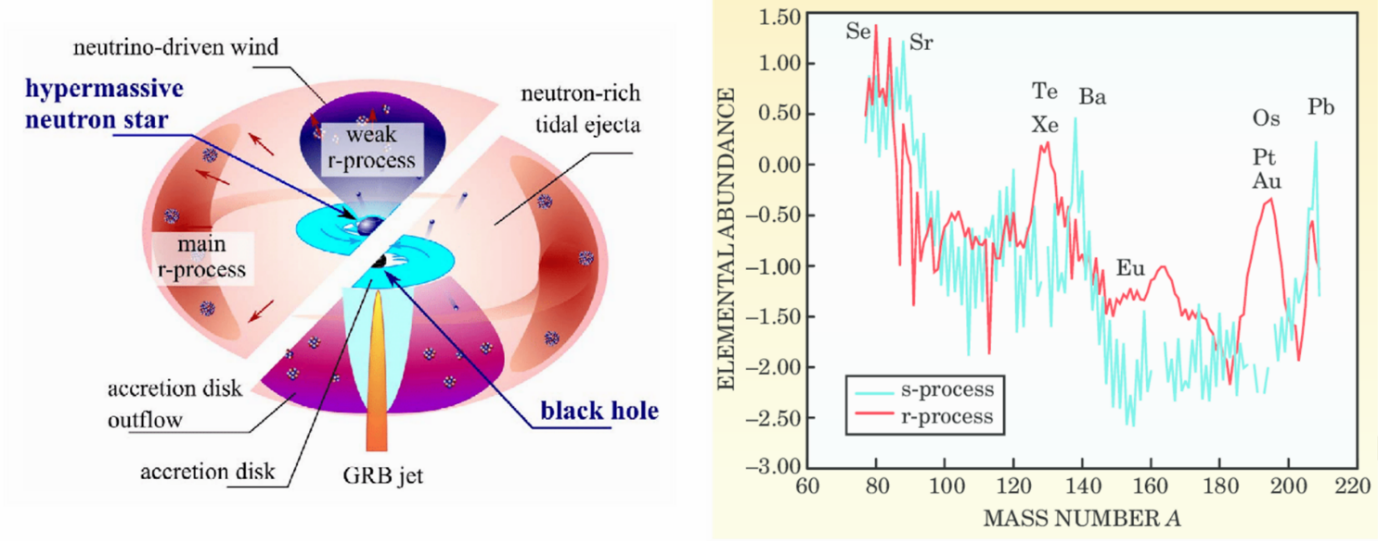
\includegraphics[width=0.85\linewidth,height=0.42\textheight,keepaspectratio]{book_media/image7.png}
\end{figure}

Fig. 7. Elements produced in collisions of compact stars

\subsection{}\label{section}

\section{Exoplanets}\label{exoplanets}

\subsection{Direct Imaging of Exoplanets Around Nearby Stars Using a Coronagraph}\label{direct-imaging-of-exoplanets-around-nearby-stars-using-a-coronagraph}

Direct imaging is one of the principal techniques for detecting and characterizing exoplanets. It involves suppressing the overwhelming light from a host star in order to isolate and observe the much fainter sources of light originating from orbiting planets. This approach makes it possible to directly visualize exoplanets whose reflected starlight or intrinsic thermal emission is typically millions to billions of times fainter than the light of their parent stars. Unlike traditional indirect detection methods---such as the radial velocity and transit techniques---direct imaging enables direct measurements of a planet's position, brightness, and spectral properties.

The key technologies underlying direct imaging are optical systems designed to suppress stellar light, such as coronagraphs and starshades. A coronagraph blocks or attenuates the stellar image within the optical system, allowing faint nearby objects---including exoplanets and circumstellar disks---to become detectable. These instruments represent one of the most important implementations of high-contrast imaging and are actively developed and employed in both space-based and ground-based observatories [63].

\textbf{Principles and Limitations of Direct Imaging}

Capturing exoplanets directly around their host stars is one of the most technically challenging methods in observational astronomy. Compared to the Sun, an Earth-like planet is typically more than a billion times fainter, making its detection extremely difficult. In addition, diffraction from the host star and wavefront aberrations within the optical system create significant obstacles to observing such faint signals. A coronagraph mitigates these effects by suppressing diffraction features and reducing scattered starlight, thereby darkening the region surrounding the star in the observer's field of view. This allows the much fainter planetary signal to become relatively more prominent.

The performance of a coronagraph is primarily characterized by two key parameters: contrast and inner working angle (IWA). Contrast represents the ratio between the detectable planetary brightness and the brightness of the host star. Modern coronagraphs and high-contrast imaging systems are being developed to achieve contrast levels as high as approximately 10⁻⁸--10⁻⁹. The IWA defines the smallest angular separation from the host star at which the coronagraph can effectively suppress starlight. A smaller IWA enables the detection of planets orbiting closer to their stars, including those with smaller orbital radii.

\textbf{Current Achievements in Direct Imaging}

Although thousands of exoplanets have been discovered to date, only a relatively small fraction have been detected through direct imaging. Nevertheless, several massive exoplanets---particularly young giant planets such as those in the HR 8799 system (HR 8799 planetary system)---have been successfully observed using this technique. These detections have been made possible through the combination of coronagraphy and advanced adaptive optics systems on large ground-based telescopes.

In 2025, reports indicated that the James Webb Space Telescope (JWST) directly detected a gas-giant exoplanet around TWA 7 using a coronagraph developed in France. This object is considered one of the lowest-mass planets ever detected through direct imaging, with a mass comparable to that of Saturn. The result demonstrates that high-contrast imaging technologies are steadily extending their capabilities toward lower-mass planets and targets located at smaller orbital separations from their host stars.

\begin{figure}[htbp]\centering
  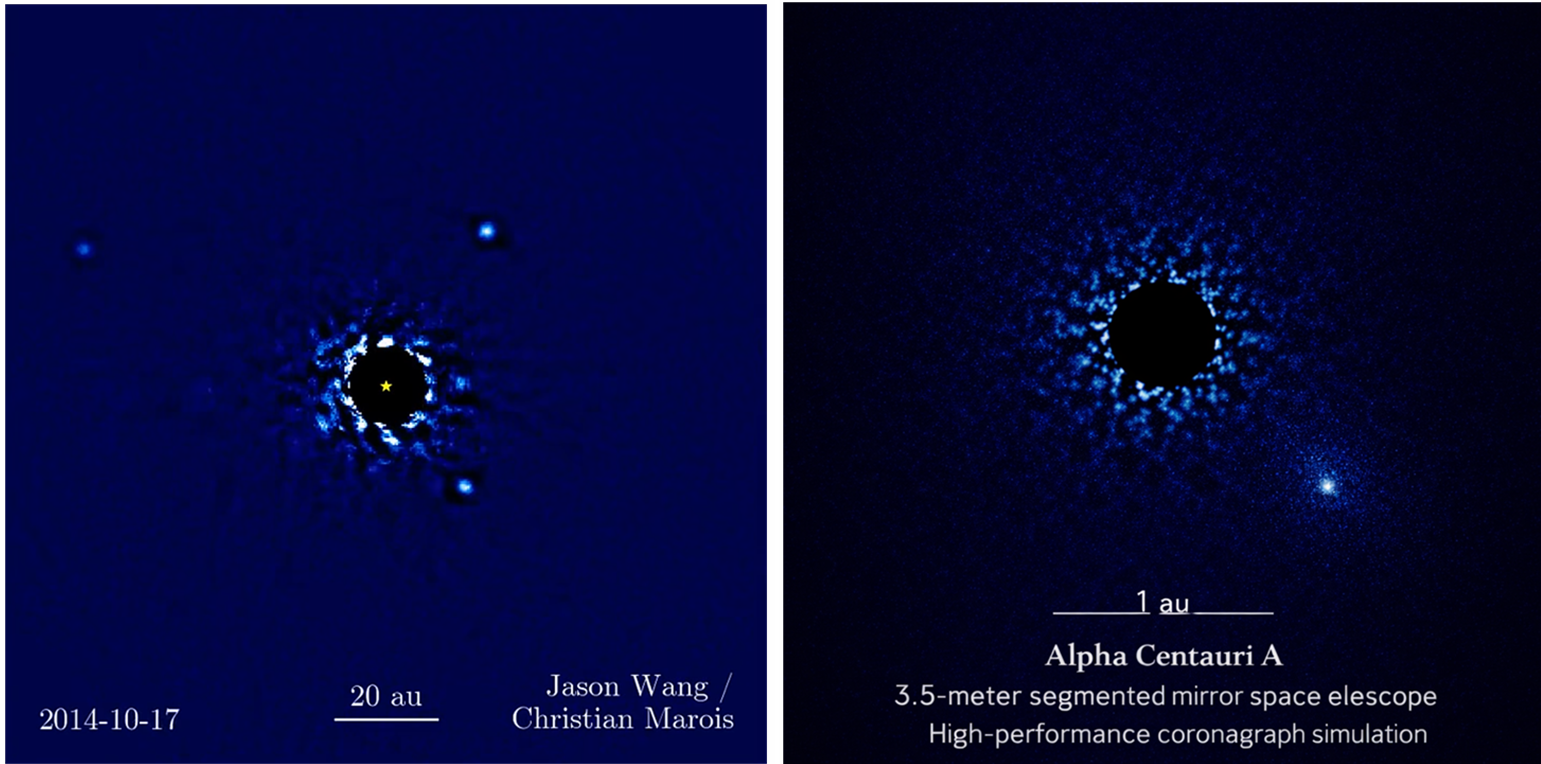
\includegraphics[width=0.85\linewidth,height=0.42\textheight,keepaspectratio]{book_media/image8.png}
\end{figure}

Fig. 8. Keck observations of HR 8799 (left) and an AI-simulated image of an exoplanet located at 1 AU from Alpha Centauri A as expected to be observed with a 3.5-meter segmented-mirror space telescope

\textbf{Direct Imaging Potential of a 3.5-Meter Space Telescope}

A 3.5-meter-class space telescope can significantly expand the applicability of direct imaging through its improved angular resolution and low-background observing environment compared with existing technologies. A space-based platform offers the advantages of being free from atmospheric turbulence and capable of achieving long integration times, making it particularly well suited for high signal-to-noise, high-contrast imaging observations. When combined with a coronagraph, a 3.5-meter telescope can provide unique capabilities in several key areas.

\begin{itemize}
\item
  \textbf{Detection of Nearby Exoplanets:}\\
  High-contrast imaging can enable the detection of exoplanets at relatively small orbital separations from their host stars, potentially down to a few astronomical units (AU) for nearby systems. This increases the possibility of directly imaging planets in closer-in orbits that are difficult to observe with current direct-imaging facilities.
\item
  \textbf{Spectroscopic Imaging and Atmospheric Characterization:}\\
  By combining a coronagraph with optical and near-infrared spectrographs, it becomes possible to investigate the atmospheric composition of detected exoplanets through the identification of molecular species such as water vapor and methane. Reflected-light spectroscopy can further reveal information about cloud properties, atmospheric structure, and planetary surface conditions. Such observations extend direct imaging beyond simple detection toward comprehensive physical characterization of exoplanets [64].
\item
  \textbf{Observations of Planet Formation and Early Evolution:}\\
  Direct imaging is particularly valuable for studying young planetary systems and stellar associations, where newly formed planets remain relatively warm and luminous. Observations at optical and infrared wavelengths can distinguish young giant planets from their host stars, providing insights into planet formation mechanisms and early evolutionary processes.
\end{itemize}

Despite these advantages, significant technical challenges remain for achieving high-performance direct imaging with a 3.5-meter-class space telescope. Wavefront control within the coronagraph system requires extremely precise optical alignment and stability. Achieving deeper contrast levels and reducing the inner working angle to access planets at smaller angular separations demand increasingly sophisticated optical architectures, wavefront-sensing techniques, and post-processing algorithms. These challenges have motivated recent theoretical investigations into advanced approaches, including quantum-information-based signal processing and methods that explore the fundamental quantum limits of high-contrast imaging [65].

\textbf{Future Prospects and Challenges}

Direct imaging is expected to advance along several important directions in the coming decades:

\begin{itemize}
\item
  \textbf{Detection of Small Planets (Earth-like and Super-Earth Planets):}\\
  The combination of large space telescopes with apertures of 3.5 meters or greater and next-generation extreme-contrast coronagraph technologies may enable observations approaching the reflected-light contrast threshold required for detecting Earth-like planets (\textgreater10⁻¹⁰). Achieving this capability would provide a powerful means of identifying potentially habitable worlds and investigating possible biosignatures.
\item
  \textbf{Atmospheric Spectroscopy and Biosignature Characterization:}\\
  Direct imaging combined with spectroscopic observations can identify molecular absorption features in planetary atmospheres, allowing detailed studies of atmospheric composition and structure. Such measurements may ultimately enable the detection of potential biosignatures and the assessment of planetary habitability.
\item
  \textbf{Multi-Method Observations and Data Integration:}\\
  Direct imaging is most powerful when combined with complementary exoplanet detection techniques, such as transit photometry and radial-velocity (RV) measurements. The integration of these observational methods can provide stronger constraints on key astrophysical parameters, including planetary mass, radius, orbital architecture, atmospheric properties, and evolutionary history.
\end{itemize}

In conclusion, direct imaging with a 3.5-meter-class space telescope has the potential to extend the current technological frontier and enable the detection and characterization of exoplanets around nearby stellar systems. Beyond the discovery of new planets, direct imaging will serve as a powerful scientific tool for investigating planetary atmospheres, physical properties, and formation histories. Continued advances in coronagraph technology, wavefront control, and high-contrast imaging systems will further enhance the precision and scientific return of future exoplanet exploration missions.

\subsection{Exoplanet Classification and Population Statistics}\label{exoplanet-classification-and-population-statistics}

In modern astronomy and astrophysics, exoplanet research has evolved beyond the simple discovery of individual planets to the systematic classification of thousands of exoplanets and the investigation of their statistical properties. Since the discovery of the first exoplanet orbiting a Sun-like star in the mid-1990s, more than 6,000 confirmed exoplanets have been identified, revealing a remarkable diversity in planetary masses, radii, and orbital characteristics (NASA Science, Exoplanets).

The goal of exoplanet classification studies is to organize these planets into meaningful groups based on their physical and orbital properties. Traditionally, exoplanets have been categorized according to their masses and radii into classes such as \textbf{rocky planets}, \textbf{mini-Neptunes}, and \textbf{gas giants}. More recently, researchers have also attempted to classify planets according to the composition of their atmospheres, inferred from absorption and reflection spectra obtained through spectroscopic observations [66].

In recent years, increasing attention has been directed toward the classification of entire planetary-system architectures. This approach considers not only the physical properties of individual planets but also the relative masses, orbital spacings, and dynamical relationships among multiple planets within the same system. Examples include \textbf{``peas-in-a-pod'' systems}, in which several similarly sized planets occupy compact orbital configurations, and systems containing \textbf{warm Jupiters}. Such classifications provide a more comprehensive description of planetary systems than classifications based solely on planetary mass or orbital period [67].

Statistical studies focus not only on the characteristics of individual exoplanets but also on determining how frequently different types of planets occur throughout the Galaxy. This field, commonly known as the \textbf{demographics of exoplanets}, seeks to measure occurrence rates and distribution functions as functions of planetary properties (such as mass and radius), orbital parameters (such as period and eccentricity), and host-star characteristics (such as spectral type) [68]. These statistical investigations provide critical constraints on theories of planet formation and evolution, helping to reveal the processes that shape planetary systems across a wide range of astrophysical environments.

\subsection{Representative Statistical Studies of Exoplanets}\label{representative-statistical-studies-of-exoplanets}

One of the most influential examples of exoplanet population studies is the \textbf{Kepler mission} conducted by NASA. From 2009 to 2013, Kepler continuously monitored approximately 190,000 stars over a period of about four years and discovered thousands of exoplanet candidates. These observations enabled researchers to estimate planetary occurrence rates based on the measured radii and orbital periods of the detected planets. The Kepler dataset demonstrated that small-radius planets are extremely common within orbital distances of roughly 1 astronomical unit (AU) and revealed that planetary systems often exhibit architectures significantly different from that of our Solar System.

Accurate statistical analyses require careful correction for \textbf{selection biases} inherent in exoplanet detection methods. Both the \textbf{transit method} and the \textbf{radial velocity method} possess sensitivities that depend on factors such as planetary size, mass, orbital inclination, and orbital period. Consequently, the observed sample cannot be directly interpreted as representative of the underlying planetary population. To derive reliable occurrence rates, probabilistic correction techniques that account for both \textbf{reliability} and \textbf{completeness} must be applied [69].

Exoplanet classification and demographic studies also play a crucial role in testing theories of \textbf{planet formation} and \textbf{planetary system evolution}. By comparing occurrence rates and classification spectra derived from multiple detection techniques with theoretical predictions, researchers can quantitatively evaluate physical processes such as protoplanetary disk mass distributions, star--planet interactions, and planetary migration. The resulting statistical patterns provide insights not only into the abundance of planets but also into the mechanisms that shape planetary systems and their long-term dynamical evolution [68].

In recent years, significant progress has been made in addressing observational biases and improving completeness corrections in exoplanet demographic studies. For example, statistical analyses of the Kepler catalog have incorporated corrections for variations in detection sensitivity and the effects of false positives, enabling the derivation of bias-corrected occurrence rates. These methods have been used to estimate fundamental population parameters, including the occurrence rate of Earth-like planets, commonly denoted as \textbf{η⊕ (eta-Earth)} [69].

Furthermore, studies of \textbf{planetary-system architectures} have become increasingly important for understanding how multiple planets are arranged and interact within a system. Such investigations examine statistical properties including orbital spacing ratios, orbital resonances, and eccentricity distributions. These measurements help characterize the typical architectures of exoplanetary systems and provide valuable constraints on theories of planetary formation, early dynamical evolution, and large-scale system organization [67].

\subsection{Astrobiological Implications and Future Prospects}\label{astrobiological-implications-and-future-prospects}

Exoplanet classification and population-statistics studies are also closely linked to \textbf{astrobiology} and investigations of \textbf{planetary habitability}. Large exoplanet datasets provide the fundamental statistical populations required for testing theories of habitability and evaluating how physical and environmental factors influence the potential for life. Such studies are essential for understanding the conditions under which habitable environments may emerge and persist on planetary bodies [70].

In summary, classification and demographic analyses based on the large samples of exoplanets discovered through both direct imaging and indirect detection techniques provide answers to a broad range of questions concerning planetary diversity, formation and evolutionary processes, and the potential existence of life under specific environmental conditions. These studies extend our understanding beyond individual planetary systems and toward a comprehensive view of planetary populations throughout the Galaxy.

Future high-performance observatories, including a \textbf{3.5-meter-class space telescope}, will greatly expand the available exoplanet sample and enable increasingly detailed demographic investigations. Improved sensitivity, higher spatial resolution, and enhanced spectroscopic capabilities will allow the detection and characterization of previously inaccessible planetary populations. Ultimately, these advances will contribute to the construction of a comprehensive map of exoplanetary ecosystems, transforming our understanding from isolated examples to a statistically robust picture of planetary systems across the Universe.

\begin{figure}[htbp]\centering
  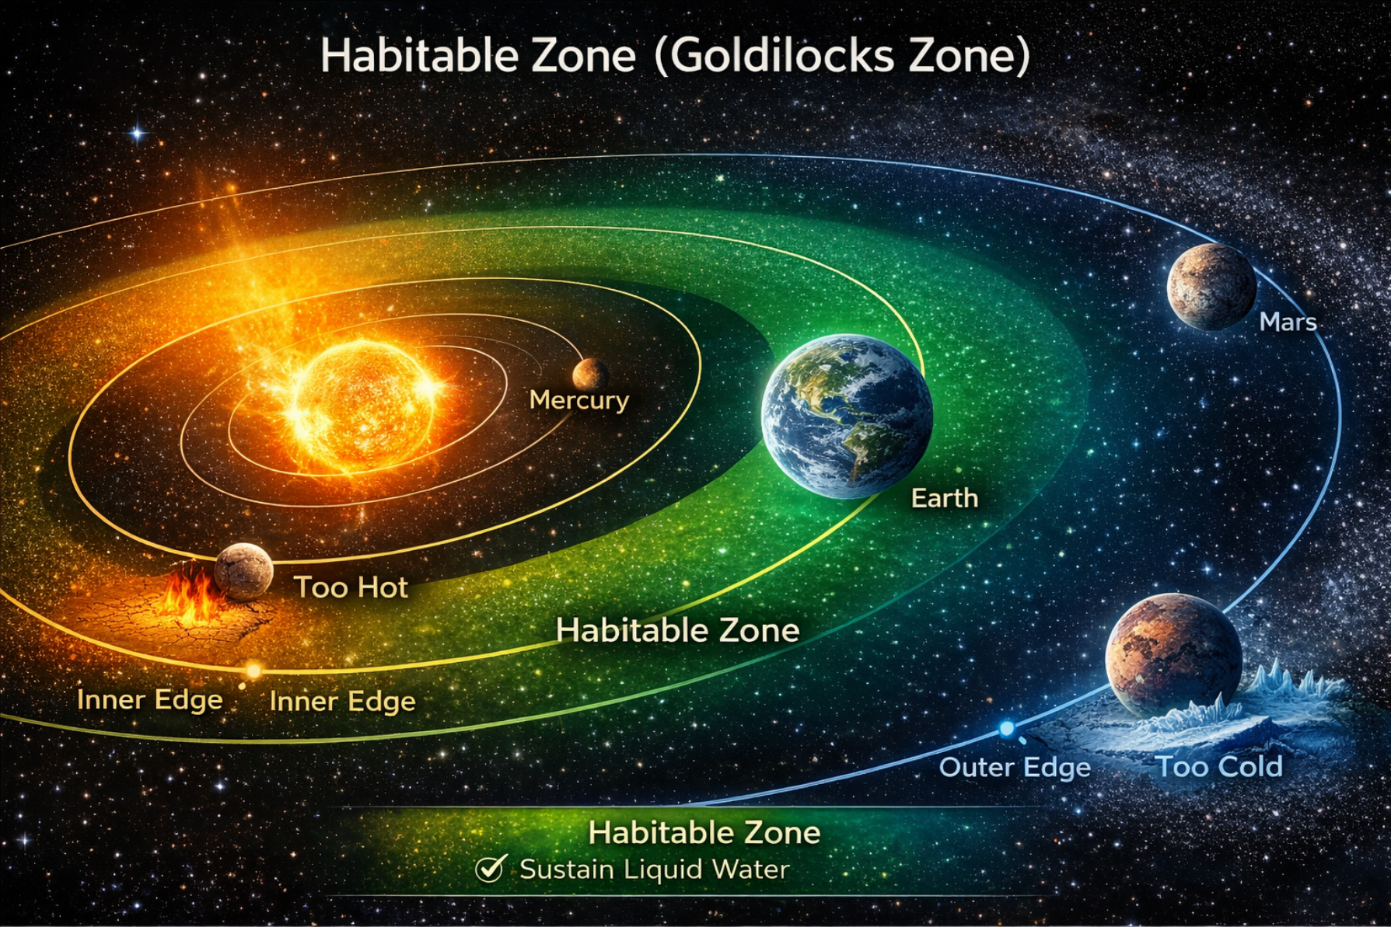
\includegraphics[width=0.85\linewidth,height=0.42\textheight,keepaspectratio]{book_media/image9.png}
\end{figure}

Fig. 9. Schematic diagram of the habitable zone in the Solar System(AI)

\subsection{Investigating the Habitability of Exoplanets}\label{investigating-the-habitability-of-exoplanets}

The study of \textbf{exoplanet habitability} is one of the most challenging and significant areas of modern astronomy. This field extends beyond merely confirming the existence of exoplanets and seeks to determine whether a planet possesses the physical, chemical, and environmental conditions necessary to support or sustain life. Habitability assessments focus on several key factors, including the potential presence of liquid water on the planetary surface, the existence of stable temperature and pressure conditions, and the detectability of atmospheric \textbf{biosignatures} that may indicate biological activity [71,72].

\subsection{Habitability and the Habitable Zone}\label{habitability-and-the-habitable-zone}

The first step in evaluating planetary habitability is to identify the \textbf{habitable zone (HZ)} around a star. The habitable zone is defined as the range of orbital distances where stellar radiation allows liquid water to exist on a planet's surface. The location and extent of the HZ depend on the spectral type, luminosity, and evolutionary stage of the host star; consequently, the HZ varies with both stellar type and age.

Planets located within the habitable zone are generally considered more likely to satisfy the basic requirement for the presence of liquid water. However, residing within the HZ alone does not guarantee habitability. Additional factors---including atmospheric composition, atmospheric retention capability, greenhouse effects, planetary geology, and the existence of a protective magnetosphere---must also be taken into account when assessing a planet's potential to support life [73].

When a planet experiences temperature conditions similar to those of Earth, liquid water may remain stable on its surface. Because of water's unique chemical properties and its role as the primary medium for known biological processes, the presence of liquid water is regarded as a fundamental requirement in most habitability studies. Nevertheless, the precise boundaries of the habitable zone are influenced by a variety of factors, including stellar ultraviolet radiation, atmospheric composition, cloud coverage, greenhouse processes, and planetary albedo. These effects are quantified through theoretical and numerical models that refine estimates of habitable-zone limits for different planetary and stellar environments [12].

\subsection{Observational Approaches: Atmospheric Spectroscopy and Biosignatures}\label{observational-approaches-atmospheric-spectroscopy-and-biosignatures}

The analysis of exoplanetary atmospheres is one of the most powerful tools for investigating planetary habitability. Certain atmospheric gases---such as \textbf{oxygen (O₂), ozone (O₃), methane (CH₄), carbon dioxide (CO₂), and water vapor (H₂O)}---are closely associated with biological processes on Earth. In particular, the simultaneous presence of oxygen and methane is of special interest because these gases tend to react with one another and are difficult to maintain together in significant quantities through purely abiotic processes. Their coexistence may therefore indicate a state of \textbf{chemical disequilibrium}, which is often regarded as a potential signature of biological activity.

Such potential indicators of life, known as \textbf{biosignatures}, can be detected through spectroscopic observations performed by space-based telescopes. Both \textbf{transit spectroscopy} and \textbf{direct-imaging spectroscopy} are valuable techniques for identifying biosignature gases within exoplanetary atmospheres [71,74]. In transit spectroscopy, starlight passes through the atmosphere of a planet during a transit event, and specific wavelengths are absorbed by atmospheric constituents. By measuring these absorption features, astronomers can infer the chemical composition and physical properties of the atmosphere. This technique has already been successfully applied to characterize the atmospheres of several giant exoplanets using facilities such as the James Webb Space Telescope.

High-contrast imaging combined with \textbf{reflected-light spectroscopy} also plays a crucial role in habitability studies. The reflected-light spectrum of a directly imaged exoplanet contains information about both its atmosphere and surface properties. Such observations can reveal the presence of water vapor, clouds, and a variety of molecular species that may be associated with habitable environments or biological activity. Because reflected-light spectroscopy can probe planetary environments in ways that complement transit observations, it is considered one of the key technologies for future large space-telescope missions dedicated to the search for habitable worlds and extraterrestrial life [75].

\subsection{Interpretation and Limitations of Biosignatures}\label{interpretation-and-limitations-of-biosignatures}

One of the most frequently discussed biosignature candidates is \textbf{molecular oxygen (O₂)}, which constitutes approximately 21\% of Earth's atmosphere and is maintained primarily through biological activity. However, oxygen can also be produced through abiotic processes under certain planetary conditions. Consequently, the detection of oxygen alone cannot be regarded as definitive evidence for the existence of life. For this reason, combinations of multiple biosignatures---such as the simultaneous detection of \textbf{O₂ and methane (CH₄)}---are generally considered more compelling indicators of biological activity. Some researchers have further proposed that the presence of a significant \textbf{thermodynamic or chemical disequilibrium} within a planetary atmosphere may itself serve as a biosignature. To investigate such possibilities, methods have been developed to compare the relative abundances of multiple molecular species and evaluate whether their coexistence can be explained through known abiotic processes [76].

Habitability studies must also carefully address the challenges of \textbf{false positives} and \textbf{false negatives}. For example, atmospheric chemical disequilibrium may arise from geological or photochemical processes rather than biological activity, leading to a false-positive interpretation of a biosignature. Conversely, life may exist on a planet without producing atmospheric signatures that are readily detectable, resulting in a false-negative outcome. Therefore, the interpretation of potential biosignatures requires the integration of multiple observational indicators and a comprehensive understanding of the planetary environment in which those signals are observed [72].

\subsection{Contributions and Prospects of a 3.5-Meter Space Telescope}\label{contributions-and-prospects-of-a-3.5-meter-space-telescope}

A \textbf{3.5-meter-class space telescope} could make significant contributions to habitability studies by providing high-resolution spectroscopic observations and broad wavelength coverage for both direct imaging and atmospheric characterization. Such a facility would be particularly well suited for investigating the atmospheres of small terrestrial planets located within the habitable zones of nearby stars, enabling atmospheric analyses with greater precision than has been achieved for many targets observed by current facilities, including the James Webb Space Telescope [73].

For example, similar in spirit to NASA's proposed Habitable Worlds Observatory (HWO), a 3.5-meter-class space telescope capable of combining advanced atmospheric spectroscopy with reflected-light spectroscopy could obtain high-quality spectral measurements of key biosignature candidates, including \textbf{oxygen (O₂), water vapor (H₂O), and methane (CH₄)}. Such observations would extend beyond simple detection by enabling comprehensive investigations of atmospheric composition, surface conditions, radiative balance, and environmental properties, thereby providing a more robust physical assessment of planetary habitability.

Furthermore, the long-term monitoring capabilities of a 3.5-meter-class telescope could offer unique opportunities to detect seasonal or climate-related variations on planets within habitable zones. Continuous observations over extended periods may reveal changes in cloud coverage, reflected-light variability, atmospheric dynamics, and weather patterns. These measurements could provide additional clues regarding environmental stability and potential ecological analogs to processes observed on Earth, thereby placing stronger constraints on planetary habitability [71].

In summary, the study of exoplanet habitability encompasses multiple interconnected components, including habitable-zone assessment, atmospheric characterization, biosignature detection, and the interpretation of observational evidence. A 3.5-meter-class space telescope represents a powerful platform for advancing all of these areas. Such investigations will move beyond the simple question of whether life exists elsewhere and toward a more comprehensive understanding of the environmental conditions and potential biological processes that may operate on planets throughout the Universe.

\subsection{Stellar Magnetic Activity and Exoplanet Habitability}\label{stellar-magnetic-activity-and-exoplanet-habitability}

\textbf{Stellar magnetic activity} encompasses a wide range of phenomena associated with stellar magnetic fields, including \textbf{starspots}, \textbf{stellar flares}, \textbf{coronal mass ejections (CMEs)}, and \textbf{high-energy X-ray and ultraviolet (XUV) radiation}. These processes can significantly influence the atmospheric composition, atmospheric retention, and surface environment of exoplanets. Their effects are particularly important in planetary systems around \textbf{M-type red dwarfs}, where the \textbf{habitable zone (HZ)} is located very close to the host star. Under such conditions, stellar magnetic activity becomes a key factor in determining planetary habitability [77,78]. Furthermore, investigating the effects of magnetic activity in young solar-type stars provides valuable insights into the evolution of Earth-like atmospheres and the environmental conditions that may have contributed to the origin of life on Earth [79].

\subsection{Effects of Stellar Magnetic Activity on Planetary Atmospheres}\label{effects-of-stellar-magnetic-activity-on-planetary-atmospheres}

One of the most prominent manifestations of stellar magnetic activity is the \textbf{stellar flare}, which releases large amounts of high-energy photons and energetic particles. These events can directly affect both the chemical structure and long-term stability of planetary atmospheres. X-rays and extreme ultraviolet (EUV) radiation emitted during flares heat the upper layers of planetary atmospheres, thereby enhancing atmospheric escape processes. If such events occur repeatedly over long timescales, the cumulative loss of atmospheric material can gradually reduce atmospheric thickness and deplete water vapor and other gases essential for maintaining habitable conditions, ultimately diminishing planetary habitability [78].

This effect is particularly severe for planets orbiting M-dwarf stars. Because the habitable zones of these stars are located at small orbital distances, planets within them are exposed to significantly higher levels of X-ray and EUV radiation, making atmospheric retention more difficult. Previous studies have shown that energetic flares from M-type stars can alter or even destroy protective atmospheric layers, such as ozone, leading to substantial long-term changes in atmospheric chemistry [11].

On the other hand, stellar magnetic activity may also have beneficial effects for the emergence of life. Previous studies suggest that energetic particles associated with stellar activity can promote \textbf{nitrogen fixation}, a process considered important for prebiotic chemistry and the development of early biological systems. Stellar activity may also contribute to the production of greenhouse gases that help maintain favorable surface temperatures [80]. In addition, energetic radiation and particle interactions may facilitate chemical pathways leading to the synthesis of amino acids and other prebiotic molecules relevant to the origin of life [81].

Therefore, the study of stellar magnetic activity is important because it exhibits a dual role in planetary evolution. While intense activity can drive atmospheric loss and reduce habitability, it may simultaneously promote chemical processes that contribute to the emergence of life. Understanding these competing effects not only provides insight into the early evolution of life on Earth but also improves our ability to interpret potential biosignatures and assess the habitability of exoplanets around a wide variety of host stars.

\subsection{Stellar Magnetic Activity and the Protective Role of Magnetospheres}\label{stellar-magnetic-activity-and-the-protective-role-of-magnetospheres}

At the planetary scale, a \textbf{magnetosphere} plays a crucial role in protecting an atmosphere from high-energy particles and radiation associated with stellar flares and other forms of stellar magnetic activity. Streams of charged particles carried by the \textbf{stellar wind} and flare-driven particle events can enhance atmospheric escape on planets with weak or absent magnetospheres. Over long timescales, such processes may lead to substantial atmospheric erosion and significant water loss, even for planets located within the habitable zone.

This effect can be particularly severe in stellar environments where \textbf{superflares} occur frequently. In such systems, the absence or weakening of a planetary magnetosphere may result in continuous atmospheric stripping, potentially creating conditions unfavorable for the emergence or long-term persistence of life. Consequently, evaluating the habitability of exoplanets requires a quantitative understanding of the interactions among stellar magnetic activity, the duration and intensity of high-energy events, and the strength and structure of planetary magnetospheres.

\subsection{Redefining the Habitable Zone in the Context of Stellar Magnetic Activity}\label{redefining-the-habitable-zone-in-the-context-of-stellar-magnetic-activity}

Traditionally, the \textbf{habitable zone (HZ)} has been defined primarily by orbital distance from the host star, based on the assumption that liquid water can exist on a planet's surface within a certain range of stellar irradiation. However, recent studies suggest that the concept of habitability should also incorporate the intensity and temporal variability of stellar magnetic activity.

Under this framework, two planets receiving similar levels of stellar radiation may experience very different environmental conditions if their host stars exhibit different levels of magnetic activity. A highly active star may subject its planets to intense flare activity, elevated XUV radiation, and enhanced stellar-wind interactions, thereby reducing the region in which stable and long-term habitable conditions can be maintained. This concept has led to the proposal of a \textbf{dynamic habitable zone}, in which habitability depends not only on stellar irradiance but also on the surrounding space-weather environment. Such an approach requires consideration of stellar age, rotation rate, magnetic-field strength, and long-term activity evolution as integral components of habitability assessments [70].

\subsection{Observational Constraints and the Need for Long-Term Monitoring}\label{observational-constraints-and-the-need-for-long-term-monitoring}

To date, many studies of stellar flares and magnetic activity have focused on individual events or relatively limited samples of stars. However, a comprehensive assessment of exoplanet habitability requires long-term observations and statistical characterization of stellar magnetic activity across a wide range of stellar types and ages. Measurements of flare frequencies, XUV radiation levels, magnetic-activity cycles, and stellar-wind properties are essential for constructing realistic atmospheric-response models and evaluating the long-term evolution of planetary environments.

A \textbf{3.5-meter-class space telescope} would provide powerful capabilities for such investigations by enabling precise monitoring of stellar magnetic activity across large and diverse stellar samples. Its high sensitivity and long-duration observing capability would allow systematic measurements of flare occurrence rates, flare energies, magnetic-activity cycles, and other indicators of stellar activity. In particular, by comparing the activity levels of stars hosting planets within their habitable zones with the observed or inferred atmospheric properties of those planets, a 3.5-meter-class space telescope could place robust quantitative constraints on the physical conditions required for planetary habitability. Such observations would contribute significantly to developing a unified understanding of how stellar magnetic environments influence the long-term evolution and potential habitability of exoplanets.

For example, potentially habitable planets orbiting M-type red dwarfs---such as Ross 128 b and Proxima Centauri b---exist within stellar environments characterized by intense flare activity, leading to ongoing debates regarding their ability to retain atmospheres and sustain conditions favorable for life. In addition, the young solar-type star EK Draconis serves as an important analogue for studying the early magnetic activity of the Sun. By combining long-term monitoring with atmospheric spectroscopic observations of such systems, a 3.5-meter-class space telescope could help establish the causal relationships between stellar magnetic activity and planetary environmental evolution.

\section{Near-Earth Objects Threatening Earth}\label{near-earth-objects-threatening-earth}

\subsection{Near-Earth Object Surveillance with a 3.5-Meter Space Telescope}\label{near-earth-object-surveillance-with-a-3.5-meter-space-telescope}

\begin{figure}[htbp]\centering
  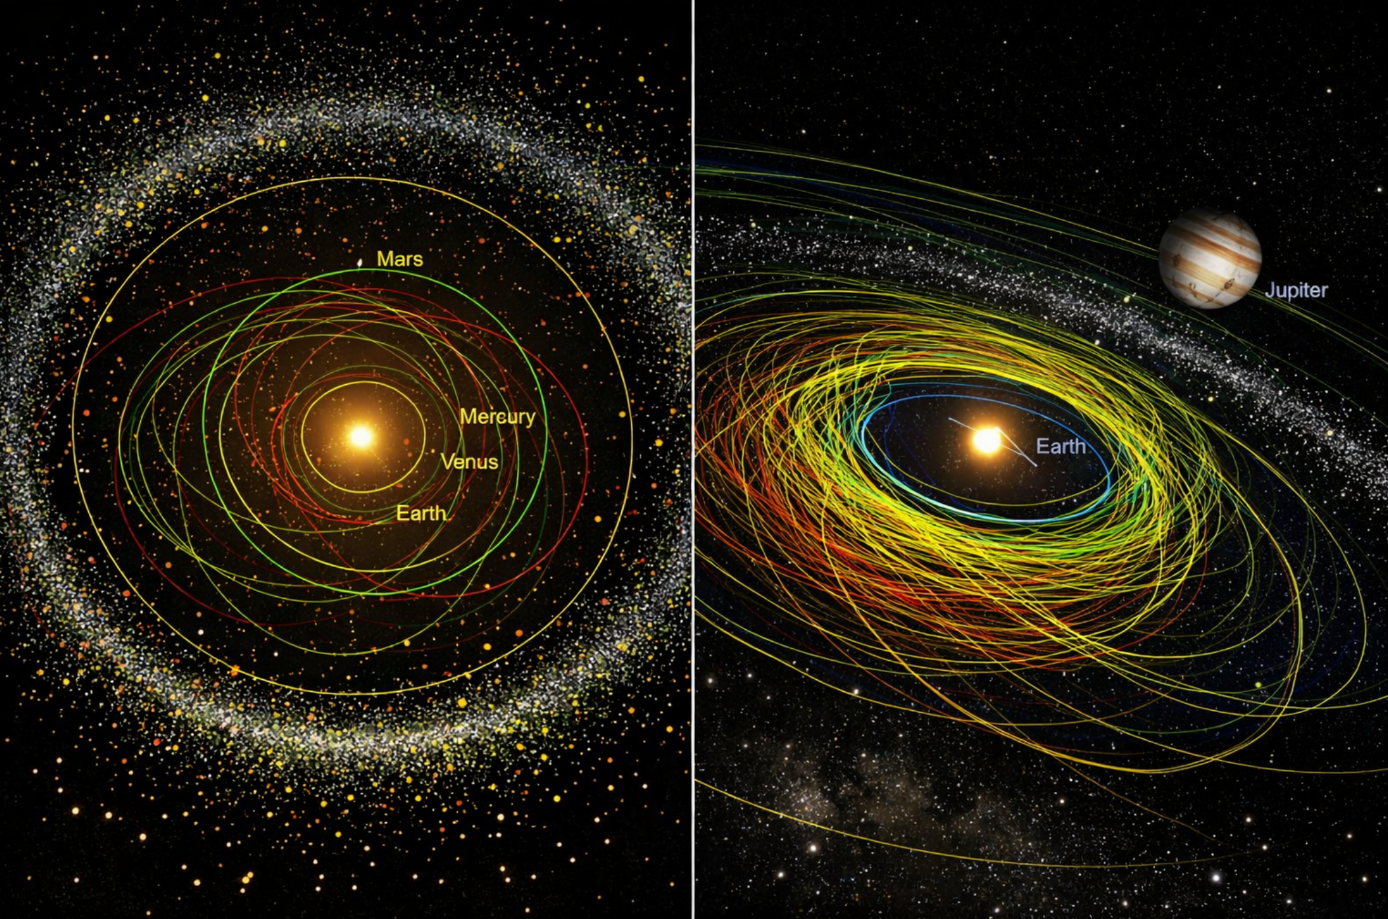
\includegraphics[width=0.85\linewidth,height=0.42\textheight,keepaspectratio]{book_media/image10.png}
\end{figure}

Fig. 10. Visualization of the distribution of more than 37,000 currently known near-Earth objects using NASA's Eyes on Asteroids(AI)

The surveillance of \textbf{Near-Earth Objects (NEOs)} is a critical area of space science aimed at ensuring the long-term safety of Earth. NEOs consist primarily of \textbf{asteroids} and \textbf{comets}, some of which have orbits that approach or intersect Earth\textquotesingle s orbit, creating a potential impact hazard. The identification, tracking, and physical characterization of potentially hazardous NEOs are essential for impact-risk assessment and the development of planetary defense strategies. The importance of this research is underscored by evidence of past impact events, such as the Chicxulub impact, which had profound consequences for life on Earth.

NEO surveillance using space-based telescopes offers significant advantages over ground-based observations. Ground observatories are constrained by atmospheric scattering, the day--night cycle, weather conditions, and seasonal visibility limitations, all of which directly affect observational efficiency. In contrast, space-based platforms operate free from these restrictions and can provide more continuous and comprehensive sky coverage. In particular, telescopes with high \textbf{infrared (IR) sensitivity} and wide-field survey capabilities are especially effective for detecting and tracking NEOs through their \textbf{thermal emission}, enabling the discovery of objects that may be difficult to detect in reflected visible light [13].

\subsection{Scientific Motivation for Near-Earth Object Surveillance}\label{scientific-motivation-for-near-earth-object-surveillance}

\begin{figure}[htbp]\centering
  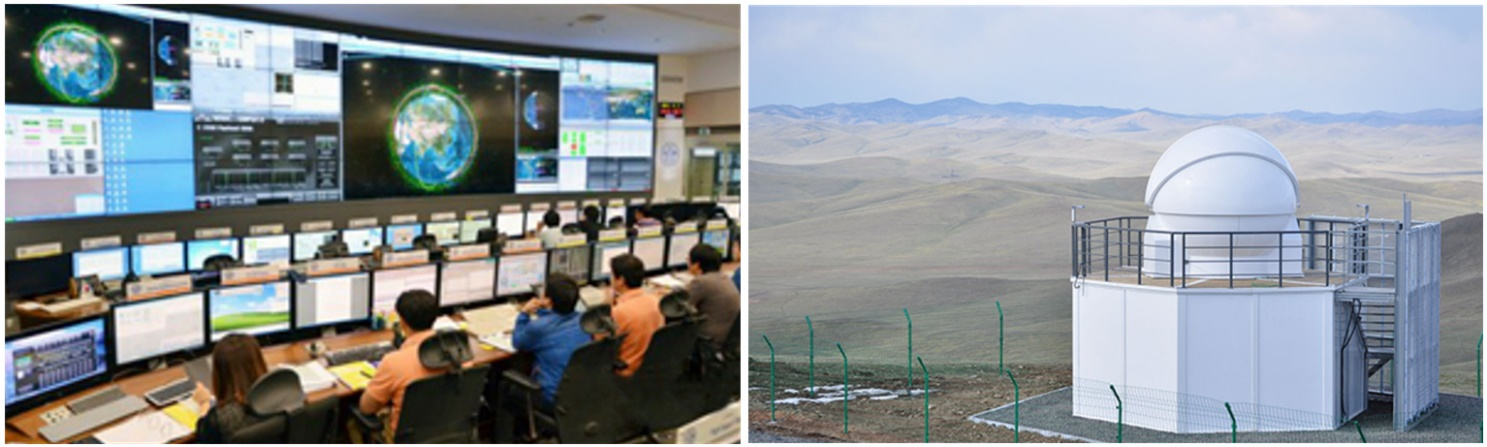
\includegraphics[width=0.85\linewidth,height=0.42\textheight,keepaspectratio]{book_media/image11.jpeg}
\end{figure}

Fig. 11. KASI's Optical Wide-field Patrol (OWL) system for space object surveillance (left). The right panel shows the OWL observatory in Mongolia.

Accurately determining the orbital and physical properties of potentially hazardous \textbf{Near-Earth Objects (NEOs)}---including their trajectories, sizes, albedos, rotation states, and surface characteristics---is the fundamental first step in assessing impact probabilities and developing effective planetary defense strategies. For NEOs with diameters ranging from several tens to hundreds of meters, the determination of orbital elements alone can often provide an initial estimate of impact risk. However, even much smaller objects, typically in the \textbf{10--30 m size range}, can produce significant regional damage upon atmospheric entry or impact. Consequently, the detection and monitoring of small NEOs remain an important scientific and societal challenge.

Most NEOs larger than approximately \textbf{100 m in diameter} are currently being discovered and tracked through ongoing survey programs. Nevertheless, a substantial fraction of objects with diameters below about \textbf{30 m} are believed to remain undetected because of observational limitations. A notable example is the Chelyabinsk meteor, a roughly 20-meter object that entered Earth's atmosphere in 2013 without prior detection and produced significant regional damage. Such events highlight the need for more comprehensive space-based NEO surveillance systems.

Observations conducted with a space telescope can simultaneously provide measurements of NEO brightness and motion across multiple wavelength bands. In particular, \textbf{infrared observations} offer a major advantage because they can detect both reflected sunlight and the object\textquotesingle s own \textbf{thermal emission}. By combining these measurements, astronomers can determine an object\textquotesingle s size and albedo with substantially greater accuracy than is typically achievable using visible-light observations alone. As a result, space-based infrared surveys provide a more reliable characterization of NEO populations and significantly improve our ability to assess potential impact hazards [44].

\subsection{Role and Capabilities of a 3.5-Meter Space Telescope}\label{role-and-capabilities-of-a-3.5-meter-space-telescope}

A \textbf{3.5-meter-class space telescope} can provide next-generation capabilities for space-based Near-Earth Object (NEO) surveillance. Its major contributions include the following:

\subsubsection{High-Sensitivity Detection and Discovery of Small NEOs}\label{high-sensitivity-detection-and-discovery-of-small-neos}

The large collecting area of a 3.5-meter telescope, combined with high-sensitivity infrared instrumentation, would significantly improve the detection of small NEOs that are difficult to observe from the ground. Compared with previous missions such as NEOWISE, the enhanced infrared sensitivity of a larger space telescope could extend detection limits to objects smaller than approximately 30 meters in diameter, thereby increasing the completeness of NEO catalogs and improving our ability to identify potentially hazardous objects before close approaches to Earth.

\subsubsection{Improved Orbital Accuracy}\label{improved-orbital-accuracy}

Space-based observations are free from atmospheric distortion and seeing effects, resulting in substantially improved astrometric precision. More accurate positional measurements allow for more precise determination of orbital elements and enhance the reliability of long-term orbital predictions. Repeated observations over extended periods further reduce uncertainties in trajectory calculations, thereby improving impact-risk assessments.

\subsubsection{Physical Characterization of NEOs}\label{physical-characterization-of-neos}

By obtaining both reflected-light and thermal-emission spectra, a space telescope can provide critical information on an object\textquotesingle s size, albedo, surface composition, and thermal properties. These physical characteristics are essential for estimating the consequences of potential impacts, understanding surface geology and material properties, and interpreting rotational and dynamical behavior. Such information also supports the design of future mitigation or deflection strategies should a hazardous object be identified.

\subsubsection{Long-Term Monitoring and Expanded Sky Coverage}\label{long-term-monitoring-and-expanded-sky-coverage}

A space-based platform can support long integration times and observations across a broad wavelength range without interruption from weather or the day--night cycle. This enables long-term monitoring programs and wide-area sky surveys that are difficult to achieve from the ground. As a result, a 3.5-meter-class space telescope can implement observational strategies that provide both extensive sky coverage and continuous tracking of newly discovered NEOs.

These capabilities would enable a more systematic and quantitative approach to \textbf{Near-Earth Object hazard assessment}. For example, accurate measurements of an NEO\textquotesingle s size, shape, and albedo can significantly improve estimates of impact energy, atmospheric entry behavior, and the geographical extent of potential damage. Consequently, a 3.5-meter-class space telescope would represent a powerful tool for advancing planetary defense and improving humanity's preparedness for future NEO impact threats.

\subsection{Technical Requirements for Near-Earth Object Surveillance}\label{technical-requirements-for-near-earth-object-surveillance}

An effective NEO surveillance system requires several key technical capabilities:

\begin{itemize}
\item
  \textbf{High-contrast imaging capability} --- the ability to separate the faint signal of small objects from the much brighter background illumination and scattered sunlight.
\item
  \textbf{Wide field of view (FOV) and high sky coverage} --- the capability to rapidly survey large areas of the sky, as NEOs are continuously moving and their positions change over time.
\item
  \textbf{Precise timing and rapid cadence observations} --- highly accurate time measurements and frequent repeated observations are essential for determining and refining the orbits of fast-moving objects.
\item
  \textbf{Adequate spectral resolution} --- sufficient spectroscopic performance is required to distinguish between reflected sunlight and thermal-emission signals, enabling the determination of physical properties such as composition, size, and surface characteristics.
\end{itemize}

In particular, \textbf{infrared spectroscopic observations} play a crucial role in accurately characterizing NEOs. Observations based solely on reflected sunlight suffer from a degeneracy between an object\textquotesingle s size and albedo: two objects with the same apparent brightness may differ significantly in their actual sizes and reflectivities. In contrast, infrared thermal-emission measurements depend directly on an object\textquotesingle s surface temperature and physical size. By combining reflected-light and thermal-emission observations, astronomers can disentangle these effects and derive more reliable estimates of size, albedo, density, and surface properties.

\subsection{Complementarity Between International Surveillance Networks and Space Telescopes}\label{complementarity-between-international-surveillance-networks-and-space-telescopes}

Current NEO surveillance efforts rely on close cooperation between ground-based survey networks and space-based observatories. A notable example of a space-based infrared survey mission is NEOWISE, while major ground-based programs such as Catalina Sky Survey, Pan-STARRS, and ATLAS continuously discover and track NEOs.

Infrared observations from space provide sensitivity to objects that are difficult to detect from the ground, particularly small and low-albedo bodies. These data complement ground-based observations and serve as valuable calibration and validation references for orbital determination and physical characterization [13].

Ground-based telescopes have the advantage of surveying large regions of the sky rapidly and at relatively low operational cost. However, their performance is inevitably affected by atmospheric conditions, weather, seeing variations, and the day--night cycle. Space-based observations are free from these limitations and benefit from darker backgrounds, longer uninterrupted observing periods, and higher signal-to-noise ratios (SNRs). The combination of ground- and space-based observations therefore represents a highly effective strategy for improving the \textbf{completeness} of NEO surveys and enabling the construction of more comprehensive catalogs that include both large and small potentially hazardous objects.

\subsection{NEO Data Processing and Impact Risk Assessment}\label{neo-data-processing-and-impact-risk-assessment}

Following NEO surveillance observations, the collected data must be incorporated into orbital-dynamics models and impact-probability calculations. Prominent examples include the NASA Jet Propulsion Laboratory \textbf{Sentry} impact-monitoring system and the European Space Agency \textbf{Near-Earth Object Coordination Centre (NEOCC)}, both of which calculate impact probabilities using the orbital elements of detected objects. Integrating NEO observations obtained from space-based telescopes with these monitoring systems can significantly improve the precision and reliability of impact-risk assessments. This demonstrates that NEO surveillance serves not only as a detection activity but also as a critical source of quantitative data for risk analysis, impact forecasting, and the development of mitigation strategies.

\subsection{Summary and Future Prospects}\label{summary-and-future-prospects}

A \textbf{3.5-meter-class space telescope} can make substantial contributions to NEO surveillance through its high sensitivity, broad wavelength coverage, long integration times, and space-based observing environment. These capabilities complement existing ground-based survey networks and are particularly valuable for the detection and characterization of small NEOs that are difficult to identify using current facilities. Beyond providing essential information for planetary defense and impact-risk assessment, such observations also contribute to our understanding of the origin, evolution, and dynamical behavior of small-body populations throughout the Solar System.

\subsection{Space Hazard Analysis of Near-Earth Objects}

\textbf{Near-Earth Objects (NEOs)} are asteroids and comets whose orbits approach or intersect that of Earth. Some of these objects pose potentially significant threats to human society and the terrestrial environment because of the possibility of impact. Consequently, research aimed at protecting Earth from such hazards has evolved beyond simple detection and tracking into a distinct and systematic field known as \textbf{space hazard analysis}.

Space hazard analysis extends beyond identifying the existence and orbital characteristics of NEOs. Its primary objective is to quantitatively evaluate and predict risk by combining the \textbf{probability} of an impact event with its potential \textbf{consequences}. Achieving this goal requires high-precision determination of an object\textquotesingle s physical properties and orbital parameters, modeling of its long-term orbital evolution, rigorous assessment of uncertainties, and the integration of these factors into comprehensive \textbf{risk metrics}. Through this approach, researchers can better characterize potential hazards and support informed decision-making for planetary defense planning and impact-mitigation strategies.

\subsection{Space Hazard Analysis: Integrating Probability, Consequences, and Systematic Risk Assessment}\label{space-hazard-analysis-integrating-probability-consequences-and-systematic-risk-assessment}

Historically, NEO research has focused primarily on the detection and orbital determination of potentially hazardous objects. However, orbital information alone is insufficient for assessing actual impact risk. Risk cannot be represented by a single value; rather, it must be treated as a function of a probability distribution that combines uncertainties in orbital predictions with outcome-related variables such as an object\textquotesingle s size, density, composition, and impact velocity.

Modern risk-analysis frameworks have developed a variety of tools to quantify the relationship between impact probability and potential consequences. Two of the most widely used approaches are the \textbf{Palermo Technical Impact Hazard Scale} and the \textbf{Torino Scale}. The Palermo Scale is a logarithmic metric designed for specialists, comparing the probability and expected impact energy of a potential collision against the background impact risk. In contrast, the Torino Scale provides a simplified rating system ranging from 0 to 10, enabling the general public and policymakers to more easily understand the significance of a potential impact threat. Through the use of such metrics, the question of \emph{``How dangerous is this object in practice?''} can be addressed in a systematic and quantitative manner rather than relying solely on the fact that an object has been discovered.

Another fundamental aspect of hazard analysis is \textbf{uncertainty propagation}. Initial observations often cover only a short observational arc, resulting in large uncertainties in the estimated orbital elements and their associated covariance matrices. As additional observations are acquired over time, these uncertainties generally decrease. However, when a close approach to Earth is anticipated, nonlinear dynamical effects become increasingly important. Consequently, simple linear covariance propagation is often insufficient. Instead, modern impact-monitoring systems employ methods that sample ensembles of possible orbital solutions throughout orbital-parameter space and search for \textbf{virtual impactors}---orbital solutions that lead to a future collision with Earth [84].

The combined evaluation of impact probability, impact consequences, and uncertainty propagation forms the foundation of quantitative space hazard analysis. Nevertheless, two major challenges remain. First, the distributions of impact consequences must be refined through improved knowledge of an object\textquotesingle s physical properties, including its size, density, shape, and albedo. Second, comprehensive dynamical models must incorporate \textbf{non-gravitational perturbations}, such as thermal forces and the \textbf{Yarkovsky effect}, which can gradually alter an object\textquotesingle s orbit over long timescales and significantly affect long-term impact predictions. Addressing these challenges is essential for improving the accuracy and reliability of future NEO hazard assessments.

\subsection{Physical Properties of NEOs and Impact Consequences: The Importance of Separating Albedo and Size}\label{physical-properties-of-neos-and-impact-consequences-the-importance-of-separating-albedo-and-size}

Traditionally, the size of a \textbf{Near-Earth Object (NEO)} is estimated from its \textbf{absolute magnitude (H)} and \textbf{albedo}. However, optical observations alone cannot uniquely determine these two quantities because the observed brightness depends on both the object\textquotesingle s size and its reflectivity. As a result, uncertainties in albedo translate directly into uncertainties in size estimates. Since the size of an NEO is a primary parameter in determining its impact energy (approximately proportional to \textbf{½mv²}), accurate size determination is essential for reliable assessments of potential impact consequences.

To overcome this limitation, observations of an NEO's \textbf{thermal emission} are required. Infrared measurements provide direct information about an object\textquotesingle s thermal radiation, allowing estimates of its surface temperature and physical size. When combined with reflected-light observations, thermal-emission data help break the degeneracy between size and albedo, enabling more accurate determination of both parameters [13]. This combined optical--infrared approach allows the estimation of absolute sizes and physical classifications that cannot be achieved through optical observations alone, thereby reducing uncertainties in impact-consequence models.

Furthermore, spectroscopic observations of reflected light can provide information on an object\textquotesingle s composition---such as whether it is dominated by silicates, carbonaceous materials, or metallic constituents---as well as its surface physical properties, including scattering behavior and surface roughness. These characteristics influence fragmentation processes, atmospheric entry dynamics, and energy-transfer mechanisms during an impact event. Consequently, they are critical inputs for \textbf{sensitivity analyses} within quantitative hazard-assessment models and for improving predictions of potential damage scenarios.

\subsection{Non-Gravitational Perturbations: The Yarkovsky Effect and Long-Term Risk Evolution}\label{non-gravitational-perturbations-the-yarkovsky-effect-and-long-term-risk-evolution}

One of the greatest challenges in long-term hazard prediction is accounting for \textbf{non-gravitational perturbations} that alter the orbits of NEOs over extended periods. Among the most important of these effects is the \textbf{Yarkovsky effect}, a mechanism in which absorbed solar radiation is re-emitted as thermal radiation, producing a small but continuous force that gradually modifies an asteroid's orbit.

Although the resulting acceleration is extremely weak, its cumulative influence can become significant over timescales of decades or longer, particularly for small NEOs. In some cases, the Yarkovsky effect can alter orbital trajectories sufficiently to change future close-approach geometries and significantly modify predicted impact probabilities.

Numerical studies have demonstrated that neglecting the Yarkovsky effect may lead to substantial inaccuracies in long-term impact-risk assessments [83]. Consequently, modern hazard-analysis frameworks increasingly incorporate Yarkovsky-related parameters or plausible ranges of thermal-force models into \textbf{Monte Carlo simulations} and long-term orbital-evolution calculations. By doing so, researchers can explore a broader range of possible future trajectories and obtain a more realistic assessment of impact probabilities than would be possible using orbital covariance propagation alone. Such approaches provide a deeper understanding of long-term NEO risk evolution and improve the reliability of future planetary-defense planning.

\subsection{The Role of a 3.5-Meter Space Telescope: From Surveillance to Hazard Analysis and Mitigation Planning}\label{the-role-of-a-3.5-meter-space-telescope-from-surveillance-to-hazard-analysis-and-mitigation-planning}

A \textbf{3.5-meter-class space telescope} has the potential to significantly strengthen multiple stages of space hazard analysis. Its contributions extend well beyond simple object detection and can be summarized as follows:

\subsubsection{1) Improving the Completeness of Early Detection}\label{improving-the-completeness-of-early-detection}

A space telescope equipped with sensitive infrared instrumentation can increase the detection rate of small NEOs that are difficult to discover using ground-based surveys alone. In particular, objects with diameters below approximately \textbf{30 m} fall within a regime where ground-based sensitivity is often limited by atmospheric effects and background noise. Space-based observations can substantially improve detection completeness in this size range by identifying objects through their thermal emission.

\subsubsection{2) Reducing Orbital Uncertainties}\label{reducing-orbital-uncertainties}

Orbital tracking relies on repeated \textbf{astrometric measurements} to refine an object\textquotesingle s trajectory and reduce uncertainties. The stable observing environment and long-term monitoring capability of a space telescope can significantly decrease the covariance associated with orbital solutions. As uncertainties shrink, families of possible orbital trajectories converge toward a smaller set of solutions, allowing potential impact scenarios to be confirmed or eliminated at much earlier stages. This improvement directly enhances the reliability of long-term impact predictions.

\subsubsection{3) Constraining Physical Properties}\label{constraining-physical-properties}

By combining optical and infrared spectroscopic capabilities, a space telescope can simultaneously measure an object\textquotesingle s size, albedo, and spectral characteristics. These measurements substantially narrow the range of input parameters used in impact-consequence calculations and hazard-assessment models. In particular, high-resolution spectroscopy can provide valuable compositional information, enabling more accurate estimates of material properties and improving models of impact-energy deposition and fragmentation behavior during atmospheric entry or surface impact.

\subsubsection{4) Constraining Non-Gravitational Perturbations}\label{constraining-non-gravitational-perturbations}

Non-gravitational effects, such as the \textbf{Yarkovsky effect}, depend strongly on an object\textquotesingle s rotational state and thermal properties. Through continuous photometric monitoring, a space telescope can obtain \textbf{rotation light curves}, allowing the determination of rotation periods, spin states, and surface thermal characteristics. These measurements provide critical inputs for thermophysical models and enable more accurate simulations of long-term orbital evolution that incorporate both gravitational and thermal forces. As a result, future trajectory predictions and impact-risk assessments become significantly more reliable.

In this way, a 3.5-meter-class space telescope would transform NEO research from a primarily detection-oriented effort into a comprehensive framework encompassing discovery, characterization, hazard analysis, and ultimately the development of informed planetary-defense and mitigation strategies.

\subsubsection{5) Providing Information for Policy and Mitigation Strategies}\label{providing-information-for-policy-and-mitigation-strategies}

The results of high-precision hazard analyses extend beyond the realm of scientific research and serve as essential inputs for policymakers and emergency-planning authorities. Accurate risk assessments enable decision-makers to establish priorities for impact mitigation, allocate resources efficiently, and develop appropriate response strategies when necessary. For example, objects assigned elevated ratings on the \textbf{Palermo Technical Impact Hazard Scale} or the \textbf{Torino Scale} may warrant immediate high-precision follow-up observations and the initiation of detailed studies on potential mitigation measures.

Taken together, these capabilities demonstrate that a \textbf{3.5-meter-class space telescope} would contribute not only to the discovery of a larger number of NEOs but also to the strengthening of a comprehensive hazard-assessment framework encompassing \textbf{detection, characterization, risk evaluation, and mitigation planning}.

\subsection{Predictive and Early Warning Analysis for Space Hazards}

Research on the detection and tracking of Near-Earth Objects (NEOs) and Potentially Hazardous Objects (PHOs) is closely connected to the broader scientific and societal objective of ensuring the long-term safety and sustainability of human civilization and the terrestrial environment. While traditional NEO studies have focused primarily on the orbital dynamics of individual objects, predictive and early warning analysis for space hazards emphasizes the early identification of potential future threats, the prediction and evaluation of risk scenarios, and the establishment of effective warning systems.

This field integrates not only information about individually detected objects but also the statistical properties of the overall NEO population, the temporal evolution of hazard events, and comprehensive modeling that combines orbital and physical characteristics. By incorporating these diverse sources of information, predictive and early warning systems aim to provide timely assessments of potential impact risks and support informed decision-making for planetary defense.

The following sections discuss the fundamental concepts of space-hazard prediction and early warning, the principal analytical and computational techniques employed in this field, the role and expected performance improvements enabled by a 3.5-meter-class space telescope, and the quantitative characteristics of such research as demonstrated through relevant studies and references.

\subsection{The Need for Space Hazard Prediction and Early Warning Systems}\label{the-need-for-space-hazard-prediction-and-early-warning-systems}

Potentially hazardous objects often possess significant orbital uncertainties at the time of their discovery. Initial observations typically cover only a \textbf{short observational arc}, making long-term orbital predictions subject to substantial uncertainty. Consequently, there is a critical need for \textbf{predictive and early warning systems} capable of identifying whether a Near-Earth Object (NEO) may pose an impact threat at some future time and of recognizing potentially hazardous scenarios as early as possible.

An effective warning system must provide a comprehensive response framework for NEO candidates whose estimated risk exceeds a specified threshold. Such a framework includes immediate and continuous follow-up observations, high-precision orbital calculations, consideration of non-gravitational perturbations, and ongoing evaluation of how impact probabilities evolve over time. Widely used hazard indicators, such as the \textbf{Palermo Technical Impact Hazard Scale} and the \textbf{Torino Scale}, are employed to quantify the severity of potential impact threats. Objects assigned Palermo Scale values above zero generally warrant additional expert review and long-term monitoring.

Importantly, an early warning system should do more than simply assign a risk rating. It must be designed to predict how impact risk may evolve in the future and to support the optimization of mitigation and response strategies as new information becomes available. A central objective is therefore the time-dependent modeling of how uncertainties in orbital elements and physical properties influence hazard metrics and risk assessments.

\subsection{Predictive and Early Warning Methodologies}\label{predictive-and-early-warning-methodologies}

\subsubsection{1) Long-Term Orbital Prediction Modeling}\label{long-term-orbital-prediction-modeling}

Reliable long-term prediction of NEO trajectories requires consideration not only of gravitational forces but also of \textbf{non-gravitational perturbations}, particularly the \textbf{Yarkovsky effect}. The Yarkovsky effect arises when solar radiation heats an object\textquotesingle s surface and the absorbed energy is subsequently re-emitted as thermal radiation, generating a small but persistent force. Although subtle, this force can accumulate over long periods and significantly alter the trajectories of small NEOs. As a result, it represents one of the principal sources of uncertainty in long-term impact predictions and must be incorporated into modern hazard-assessment models.

Numerous studies have demonstrated that multivariate \textbf{Monte Carlo simulations} incorporating the Yarkovsky effect can substantially improve the accuracy of long-term impact-risk forecasts [83]. Such simulations require a nonlinear probabilistic framework that simultaneously accounts for uncertainties in the orbital \textbf{state vector}, non-gravitational perturbation parameters, observational errors, and the temporal spacing of observations.

A common approach involves generating large ensembles of \textbf{virtual clones} representing plausible orbital solutions within the uncertainty region of the observed orbit. Each clone is then propagated forward in time to determine its future trajectory and minimum Earth-approach distance. By analyzing the statistical behavior of these orbital ensembles, researchers can estimate the time evolution of impact probabilities and identify periods of elevated risk. This methodology typically follows the sequence:

\textbf{Input Uncertainties → Impact Probability Distribution → Prediction of Warning and Risk-Escalation Timelines}

Such an approach provides a quantitative foundation for future early warning systems and enables more reliable long-term forecasting of potential NEO impact hazards.

\subsection{2) Integrated Risk Scales and Warning Criteria}\label{integrated-risk-scales-and-warning-criteria}

The \textbf{Palermo Technical Impact Hazard Scale} and the \textbf{Torino Scale} are the most widely used tools for impact-risk assessment. The Palermo Scale expresses risk as a logarithmic measure that combines impact probability with expected impact energy, facilitating quantitative comparisons among potential threats by specialists. The Torino Scale, in contrast, is designed for public communication and provides a simplified classification system that combines impact probability and potential consequences into a single risk level.

For example, objects assigned a \textbf{Torino Scale value of 2 or higher} generally warrant additional observations and are often interpreted as representing a temporary warning level. Objects reaching \textbf{Torino Scale values of 5 or higher} are typically considered significant enough to justify substantial scientific attention and preparedness planning. Together, these scales provide a common framework for translating complex impact-risk assessments into standardized warning indicators.

\subsection{Role of a 3.5-Meter Space Telescope and Expected Performance Improvements}\label{role-of-a-3.5-meter-space-telescope-and-expected-performance-improvements}

A \textbf{3.5-meter-class space telescope} has the potential to substantially enhance multiple stages of predictive and early-warning research for space hazards. Its major contributions can be summarized as follows:

\subsubsection{(A) Improved Detection and Reduction of Initial Uncertainties}\label{a-improved-detection-and-reduction-of-initial-uncertainties}

The large collecting area and high sensitivity of a space telescope enable the discovery of smaller NEOs and facilitate rapid initial orbit determination. The positional uncertainties associated with short observational arcs immediately after discovery can be significantly reduced through space-based astrometric observations. This improvement directly reduces the initial uncertainty space used in long-term probability simulations and impact-risk assessments [84].

\subsubsection{(B) Expanded Physical Characterization}\label{b-expanded-physical-characterization}

By combining optical and infrared observations, a space telescope can simultaneously determine an NEO's size, albedo, and spectral composition. These parameters constitute critical inputs for impact-consequence models. In particular, the combined analysis of reflected and thermal radiation breaks the degeneracy between size and albedo, significantly reducing uncertainties in estimates of impact energy and potential damage [13].

\subsubsection{(C) Improved Long-Term Orbital Predictions}\label{c-improved-long-term-orbital-predictions}

Long-term monitoring over periods ranging from years to decades can substantially improve orbit determination. Repeated high-precision astrometric measurements allow the detection of subtle orbital changes caused by non-gravitational perturbations. By constraining these effects and incorporating them into orbital-evolution models, a 3.5-meter-class space telescope can greatly reduce uncertainties in long-term hazard forecasts [83].

\subsubsection{(D) Identification of Critical Warning Thresholds}\label{d-identification-of-critical-warning-thresholds}

One of the most important objectives of an early-warning system is determining when a risk metric exceeds a predefined threshold. By providing highly accurate observations that constrain the initial conditions of long-term orbital simulations, a 3.5-meter-class space telescope can identify such threshold crossings at earlier stages. Earlier detection of elevated risk levels increases the time available for scientific assessment, policy development, and potential mitigation planning.

\subsubsection{(E) Multi-Signal Observations and Hazard Information Integration}\label{e-multi-signal-observations-and-hazard-information-integration}

Observations obtained by a 3.5-meter-class space telescope can be integrated with ground-based optical and radar measurements as well as data from other space missions, such as the James Webb Space Telescope. Such multi-platform data fusion can substantially improve the accuracy of impact-risk assessments. For example, combining radar-derived distance and velocity measurements with space-based physical characterization data yields more precise orbital solutions and more reliable long-term predictions.

\subsection{Expected Outcomes and Applications}\label{expected-outcomes-and-applications}

Predictive and early-warning research for space hazards provides benefits that extend far beyond the issuance of impact alerts. Comprehensive time-dependent risk models can forecast the evolution of impact probabilities over periods spanning decades and identify when and where critical risk thresholds may emerge. These predictive risk maps can serve as valuable decision-support tools for public policy, emergency management, and disaster-preparedness planning.

In addition, long-term observational datasets contribute to studies of \textbf{NEO population statistics} and the overall structure of small-body populations in the Solar System. By revealing the spatial and temporal distributions of cumulative risk, these datasets improve our understanding of how hazardous-object populations evolve and help refine the methodologies used to estimate impact risk. Ultimately, such research contributes not only to planetary defense but also to the broader scientific understanding of the dynamical evolution of near-Earth object populations.

\chapter{Mission Operations}\label{mission-operations}

\section{Orbit}\label{orbit}

The 3.5-meter segmented-mirror robotic space telescope is planned to operate either at the Sun--Earth L2 point (approximately 1.5 million km from Earth) or in a low Earth orbit (LEO) at an altitude of about 700 km. Both orbital options provide several common advantages, including a thermally stable environment, low-radiation conditions, continuous access to a large fraction of the sky, and reliable communication with ground stations. The mission is expected to support the downlink of several tens of gigabytes of scientific data per day while enabling rapid responses to unexpected external events and transient astronomical phenomena. However, if the telescope is deployed at L2, the role of AI-based robotic operations will become particularly important due to the greater distance and limited opportunities for direct human intervention.

Several orbital candidates were evaluated for the 3.5-meter segmented-mirror robotic space telescope, including geostationary orbit (GEO), the Sun--Earth L2 point, an Earth-trailing heliocentric orbit, and various medium Earth orbits (MEOs). The trade-off analysis considered multiple factors, including radiation exposure, the duration and frequency of eclipses, the effects of Earth infrared emission and reflected sunlight (albedo) on thermal stability, achievable data downlink rates as a function of distance, and the complexity of final orbit insertion maneuvers. Based on this assessment, we propose either the Sun--Earth L2 point (approximately 1.5 million km from Earth) or a low Earth orbit at an altitude of about 700 km as the most suitable operational orbit for the mission.

\begin{figure}[htbp]\centering
  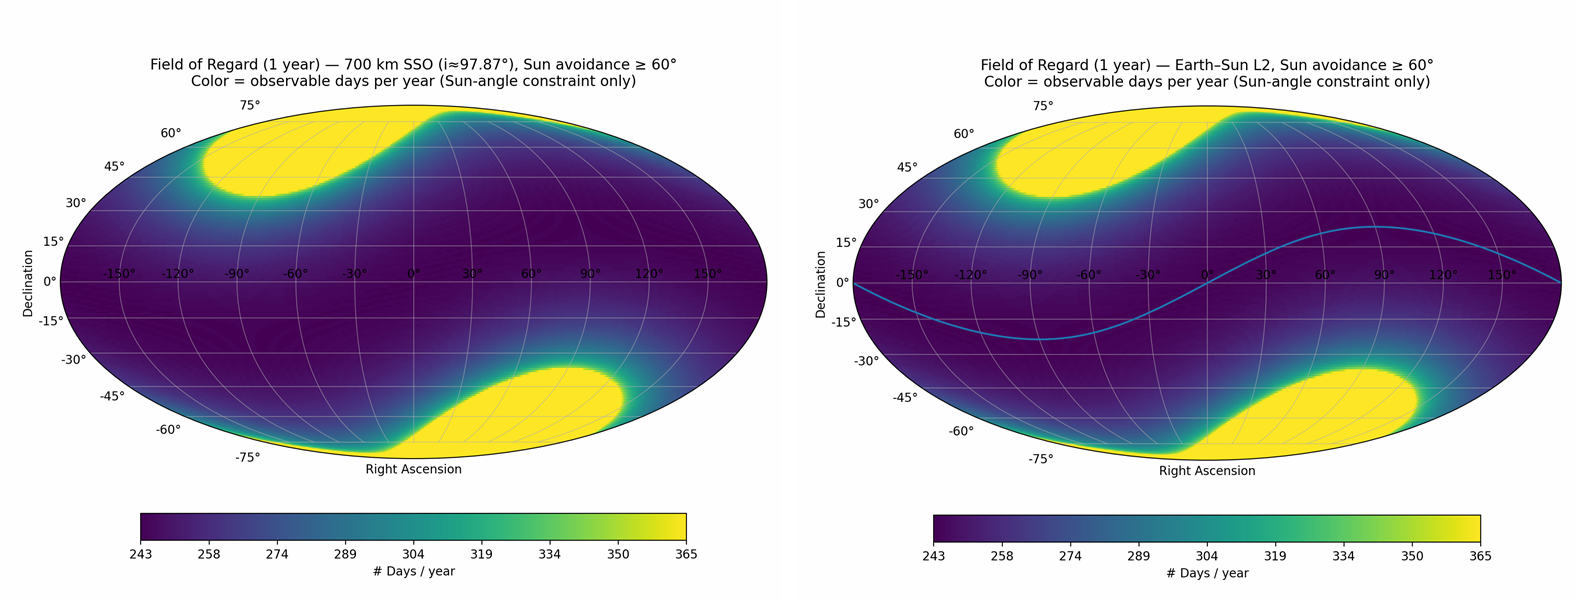
\includegraphics[width=0.85\linewidth,height=0.42\textheight,keepaspectratio]{book_media/image12.png}
\end{figure}

Fig. 12. The above figure illustrates the field of regard of the 3.5-meter space telescope for operation in a 700 km Sun-synchronous orbit (SSO) (left) and at the Sun--Earth L2 point (right). The color bar represents the annual number of observable days corresponding to each color, ranging from 243 days near the ecliptic plane to 365 days near the ecliptic poles for both orbital configurations(AI).

These orbital environments have already been well demonstrated by previous space missions and are expected to provide high downlink capacity and excellent spacecraft stability. They offer access to nearly the entire sky, while their stable orbital characteristics minimize the need for station-keeping maneuvers, thereby reducing propellant consumption and extending the operational lifetime of the mission. In particular, the L2 orbit requires only minimal station-keeping and does not necessitate a dedicated disposal maneuver at the end of the mission.

The left panel of Figure 13 does not explicitly represent the characteristics of a Sun-synchronous orbit (SSO), such as its orbit--Sun geometry. Instead, it is more accurately interpreted as a map of the annual observable days for a space telescope operating under a solar avoidance angle constraint of 60°, regardless of its specific orbit. The Field of Regard was calculated by counting the number of days during which the angular separation between a target and the Sun is greater than or equal to 60°. Under this condition, the theoretical minimum visibility is approximately 243 days per year for targets near the ecliptic plane, while the maximum visibility reaches 365 days per year for targets near the ecliptic poles. The right panel shows the corresponding result for an observatory operating at the Sun--Earth L2 point, yielding essentially the same visibility distribution.

\section{Operations Concept}\label{operations-concept}

The operations concept of the 3.5-meter segmented-mirror robotic space telescope is founded on two key principles: \textbf{automation-first operations} and \textbf{rapid-response capability}. Unlike traditional space observatories that rely primarily on long-term, static observing schedules, this mission aims to establish a flexible and dynamic observing framework suitable for the era of time-domain and multi-messenger astronomy. In particular, the entire operational architecture is designed from the outset to support rapid follow-up observations of time-critical astrophysical phenomena---including gravitational-wave events, gamma-ray bursts, rapidly evolving supernovae, and active galactic nucleus (AGN) flares---within timescales of only a few hours.

Ground operations are divided into two primary components: the \textbf{Science Operations Center (SOC)} and the \textbf{Mission Operations Center (MOC)}. The SOC is responsible for observation proposal management, long- and short-term observation planning, Target of Opportunity (ToO) validation, and science data processing and distribution. The MOC oversees spacecraft operations, attitude control, command uplink, health monitoring, and safe mission execution. These two operational entities are tightly integrated through real-time or near-real-time information exchange, enabling automated reprioritization of observing programs and rapid telescope repointing whenever urgent observation requests are received.

A central element of the mission architecture is an intelligent \textbf{dynamic queue scheduling} system. All observing programs are managed within a multidimensional framework that incorporates scientific priority, timing constraints, solar avoidance requirements, spacecraft attitude limitations, thermal stability conditions, instrument status, and data downlink opportunities. Based on these constraints, the scheduling system continuously recalculates observing plans on short timescales. This approach is designed to maximize overall scientific productivity while maintaining an appropriate balance among large long-term programs, precision time-series monitoring, recurring observing campaigns, and high-priority ToO observations.

Rapid ToO response constitutes one of the mission's primary requirements. The observatory is designed to initiate observations of scientifically justified high-priority events within a few hours whenever possible. To achieve this capability, the operational framework incorporates end-to-end automation, including automated alert ingestion, onboard schedule patching, rapid spacecraft repointing, and automatic generation of observation sequences. The baseline operational goal is to provide reliable ToO response within approximately 12 hours, while selected high-priority events may receive conditional rapid-response observations within approximately 4 hours. These performance goals are defined within the practical constraints imposed by orbital geometry, solar avoidance angles, thermal stabilization requirements, and communication visibility.

The mission architecture is also designed for integration with international time-domain and multi-messenger observing networks. External alerts originating from gravitational-wave detectors, neutrino observatories, and high-energy astrophysical monitoring systems are automatically ingested and evaluated through predefined validation procedures. When warranted, ongoing observations may be interrupted and replaced by emergency follow-up programs. In addition, the science data processing system includes a quick-look pipeline for preliminary quality assessment, enabling rapid dissemination of observational results and timely data sharing with international collaboration networks during significant transient events.

Over the long term, the mission aims to evolve toward a highly autonomous robotic observatory. To support this objective, advanced capabilities such as repetitive observation pattern analysis, priority-based optimization algorithms, and constraint-driven schedule reconstruction will be introduced progressively. The potential application of machine-learning-assisted decision-support techniques is also under consideration. Nevertheless, operational transparency, reliability, and safety remain the highest priorities. Consequently, the initial operational phase will adopt a conservative approach based on well-established rule-based scheduling systems operating under continuous human supervision.

Beyond improving observational efficiency, this operations concept establishes the foundation for the 3.5-meter segmented-mirror robotic space telescope to serve as a major space-based follow-up facility in the era of international time-domain astronomy. By integrating long-duration high-precision observations with rapid-response capabilities within a single observatory, the mission is designed to provide both exceptional scientific flexibility and sustained long-term value for future space astronomy research.

\chapter{Conclusion}

The 3.5-meter segmented-mirror robotic space telescope has been proposed to address an increasingly evident observational gap in contemporary and near-future astrophysical research. As the era of time-domain and multi-messenger astronomy continues to expand, the demand for a large-aperture space-based optical and near-infrared observatory capable of combining rapid-response observations, long-term high-stability spectrophotometry, and broad wavelength coverage is growing rapidly. Existing and planned space observatories have generally been optimized for specific scientific objectives and operational philosophies, leaving relatively few facilities capable of simultaneously providing responsiveness, stability, versatility, and operational flexibility.

Within this context, the proposed 3.5-meter space telescope is designed to serve a complementary role alongside existing and future observatories by integrating a large-aperture segmented-mirror optical system, purpose-driven scientific instrumentation, and an automation-centered rapid-response operational framework. The mission is not intended merely to achieve greater collecting area or higher angular resolution, but rather to realize a highly agile space observatory capable of delivering the right observations at the moments when they are scientifically most valuable.

The scientific reach of the observatory extends across a broad range of disciplines, including time-domain and multi-messenger astronomy, exoplanet characterization, compact-object astrophysics, galaxy evolution, and precision cosmology. Its ability to provide continuous optical-to-near-infrared spectrophotometry, high-precision multi-band imaging, long-term time-series observations, and selective high-contrast coronagraphic observations within a single platform opens new avenues for investigating rapidly evolving astrophysical phenomena. In particular, the mission has the potential to become a key follow-up facility within international observing networks for time-critical science cases such as gravitational-wave counterparts, the earliest phases of supernova explosions, active galactic nucleus variability, and exoplanet atmospheric characterization.

The observatory is also conceived not as a standalone facility, but as a network-oriented space observatory operating in close coordination with wide-field time-domain surveys such as the Rubin Observatory, next-generation gravitational-wave detectors, infrared space telescopes, and high-energy astrophysical missions. This design philosophy reflects the reality that modern astronomy increasingly advances through cooperation among multiple facilities and the integration of heterogeneous datasets rather than through competition among individual observatories. Within such an international framework, the mission would enable the Republic of Korea not merely to participate in global scientific collaborations but to contribute a major observational asset to the worldwide astronomical community.

Beyond its scientific objectives, the 3.5-meter space telescope also serves as a strategic testbed for future approaches to the development and operation of large space observatories. The mission proposes an alternative pathway to the traditional flagship model characterized by multi-decade development schedules and extremely high costs. Instead, it embraces a framework that combines managed risk acceptance, accelerated deployment, software-enabled operations, and an open-science philosophy. This approach is not primarily motivated by cost reduction but by the desire to deploy scientifically relevant observational capabilities while the most compelling scientific questions remain timely and actionable.

The mission further incorporates advanced operational concepts, including automated dynamic scheduling, rapid Target-of-Opportunity response, reproducible scientific analysis environments, open-access archives, and software-centered data ecosystems. These capabilities position the observatory as a pathfinder for future transformations in space astronomy operations. The operational philosophy developed through this mission may ultimately provide valuable guidance for the design and management of next-generation space-based observatories over the coming decades.

From a national perspective, the significance of this mission is equally substantial. As the first large-aperture space astronomy platform independently designed, developed, and operated by the Republic of Korea, the 3.5-meter space telescope represents more than a scientific instrument; it symbolizes a structural advancement in the nation's space science capabilities. The technologies and expertise accumulated through the mission---including segmented-mirror systems, high-stability space optics, precision space-based observing operations, and large-scale data and software ecosystems---will form a critical foundation for future flagship observatories and deep-space scientific missions. The project will also provide long-term opportunities for both the domestic research community and industrial partners to assume more influential roles in international space astronomy programs.

Taken together, these factors suggest that the 3.5-meter segmented-mirror robotic space telescope has the potential to become far more than a single scientific mission. It represents a next-generation space observatory platform capable of delivering both significant scientific impact and strategic value in the post-2030 space astronomy landscape. By simultaneously linking scientific discovery, operational innovation, international collaboration, and national capability development, the mission offers a new model for future space observatories and may mark an important milestone in the transition of Korean astronomy into the era of space-based flagship observational facilities.

\textbf{Acknowledgements}

This work was supported by the 2026 Korea Astronomy and Space Science Institute (KASI) major research program, ``Development of Advanced Laser Interferometry Technologies for Participation in the International Joint Development of Next-Generation Gravitational-Wave Detectors'' (Project No. 2026181000).

\chapter*{References}\addcontentsline{toc}{chapter}{References}

1. Abbott BP, Abbott R, Abbott TD, et al., GW170817: Observation of gravitational waves from a binary neutron star inspiral, Phys Rev Lett 119:1101.Seager (2017).

2. Margutti R, et al., An embedded X-ray source shines through the aspherical AT2018cow: Revealing the inner workings of the most luminous fast-evolving optical transients, ApJ 872:18. (2019).

3. Prentice SJ, et al., The Cow: Discovery of a luminous, hot, and rapidly evolving transient, ApJ 865:L3. (2018).

4. LSST Science Collaboration, et al., LSST Science Book, Version 2.0, arXiv:0912.0201. (2009).

5. Roman Space Telescope Science Team., Nancy Grace Roman Space Telescope: Science objectives and mission overview, [Internet], viewed 2026 May 23, available from: \url{https://www.stsci.edu/roman}

6. Ivezić Ž, et al., LSST: From science drivers to reference design and anticipated data products, ApJ 873:111. (2019).

7. Zurlo, A, Direct imaging of exoplanets, arXiv:2404.05797. (2026).

8. Riess AG, et al., Observational evidence from supernovae for an accelerating universe and a cosmological constant, AJ 116:1009. (1998).

9. Perlmutter S, et al., Measurements of Ω and Λ from 42 high-redshift supernovae, ApJ, 517, 565P. (1999).

10. Planck Collaboration., Planck 2018 results. VI. Cosmological parameters, A\&A, 641, A6 (2020).

11. Chen H, Zhan Z, Youngblood A, et al., Modeling stellar activity and its effects on exoplanet atmospheres and habitability, Nat Astron 5:298. (2021).

12. Seager S., Exoplanet habitability, Science 340:577. (2013).

13. Mainzer A, Grav T, Bauer J, et al., NEOWISE observations of near-Earth objects: Preliminary results, ApJ 743:156. (2011).

14. NASA Planetary Defense Strategy 2023, [Internet], viewed 2026 May 23, available from:

\url{https://science.nasa.gov/planetary-defense/}

15. Roos M., Introduction to Cosmology, arXiv:1001.0316. (2010).

16. Arbey A, Mahmoudi F., Dark Matter and the Early Universe: A Review, Prog Part Nucl Phys 119:103865. (2021).

17. Rubakov VA., The Null Energy Condition and its Violation, Physics-Uspekhi, 57, 128--142 (2014)

18. Billard J, Boulay M, Cebrián S, et al., Direct Detection of Dark Matter --- APPEC Committee Report, Rep Prog Phys 85:056201. (2022).

19. Akrami Y, et al. (Planck Collaboration)., Planck 2018 Results. X. Constraints on Inflation, A\&A 641:A10. (2020).

20. Baumann D., TASI Lectures on Inflation, in Physics of the Large and the Small, TASI 2009, World Scientific, 2011.

21. Peebles PJE., The large-scale structure of the universe, Princeton University Press, Princeton, NJ. (1980).

22. Dodelson S., Modern cosmology, Academic Press, San Diego, CA. (2003).

23. Springel V, et al., Simulations of the formation, evolution and clustering of galaxies and quasars, Nature 435:629--636. (2005).

24. Schramm DN, Turner MS., Big-bang nucleosynthesis enters the precision era, Rev Mod Phys 70:303. (1998).

25. Tegmark M, et al., Cosmological parameters from SDSS and WMAP, Phys Rev D 69:103501. (2004).

26. Komatsu E, et al., Seven-Year Wilkinson Microwave Anisotropy Probe (WMAP) Observations: Cosmological Interpretation, ApJS 192:18. (2011).

27. Bartolo N, et al., Non-Gaussianity from inflation: Theory and observations, Phys Rep 402:103. (2004).

28. Meerburg PD, et al., Primordial gravitational waves, BAAS 51(3):107. (2019).

29. Kamionkowski M, Kovetz ED., The quest for B modes from inflationary gravitational waves, Annu Rev Astron Astrophys 54:227. (2016).

30. Furlanetto SR, et al., Cosmology at low frequencies: The 21 cm transition and the high-redshift Universe, Phys Rep 433:181. (2006).

31. Pritchard JR, Loeb A., 21 cm cosmology in the 21st century, Rep Prog Phys 75:086901. (2012).

32. Ahn K., How Model Variance in High-Redshift Star Formation Shapes Cosmic Reionization History, PKAS 34:67. (2019)

33. Farcy M, et al., The impact of cosmic ray feedback during the epoch of reionisation, A\&A 698:A89. (2025).

34. Raaijmakers G., et al., Constraints on the Dense Matter Equation of State and Neutron Star Properties from NICER's Mass--Radius Estimate of PSR J0740+6620 and Multimessenger Observations, ApJL 918:L29. (2021).

35. Smith A., Kannan R., Garaldi E., Vogelsberger M., Pakmor R., Springel V., Hernquist L., The thesan project: Lyman-α emission and transmission during the, MNRAS, 512, 3243 (2022)

36. Siegel, G., and et al. The Suppression of the Matter Power Spectrum: Strong Feedback from X-ray Gas Mass Fractions, kSZ Effect Profiles, and Galaxy-galaxy Lensing." arXiv preprint arXiv:2512.02954.(2025)

36. Salaris M, et al., The Cooling of CO White Dwarfs: Influence of the Internal Chemical Distribution, ApJ 486:413. (1997).

37. Córsico A. H., White-dwarf asteroseismology: an update, arXiv:1912.06738, (2019)

38. Bédard A, The spectral evolution of white dwarfs: where do we stand?, Astrophysics and Space Science, 369:43, (2024)

39. Córsico, A. H., White-dwarf asteroseismology with the TESS space telescope, BAAA, 63, 48, (2022)

40. Zuckerman B, Becklin EE., Excess infrared radiation from a white dwarf, Nature 330:138. (1987).

41. Koester D, Gänsicke BT, Farihi J., The frequency of planetary debris around young white dwarfs, A\&A 566:A34. (2014).

42. Debes J, Walsh K, Stark C., The link between planetary systems, dusty white dwarfs, and metal-polluted white dwarfs, ApJ 747:9. (2012).

43. Farihi J, Barstow MA, Redfield S, Dufour P, Hambly NC., Rocky planetary debris around white dwarfs, MNRAS 404:2123. (2010).

44. Vanderburg A, et al., A disintegrating minor planet transiting a white dwarf, Nature 526:546. (2015).

45. Guidry JA, et al., Direct imaging mission yield estimates for nearby planetary systems, ApJ 912:125. (2021).

46. S. Xu, K. Y. L. Su, L. Rogers, A. Bonsor, J. Olofsson, D. Veras, R. van Lieshout, P. Dufour, E. M. Green, E. Schlawin, et al., Infrared Variability of Two Dusty White Dwarfs, The Astrophysical Journal, 866:108 (2018)

47. Xu S, et al., Compositions of Planetary Debris around Dusty White Dwarfs, AJ 158:242. (2019).

48. Rafikov RR, Metal Accretion onto White Dwarfs Caused by Poynting--Robertson Drag on Their Debris Disks, The Astrophysical Journal Letters, 732:L3 (2011).

49. Rocchetto M, Farihi J, Gänsicke BT, Bergfors C., The frequency and infrared brightness of circumstellar discs at white dwarfs, MNRAS 449:574. (2015).

50. Lattimer JM, Prakash M., Phys Rep, Neutron star observations: Prognosis for equation of state constraints, Physics Reports, 442:109--165 (2007).

51. Özel F, Freire P., Masses, radii, and the equation of state of neutron stars, Annu Rev Astron Astrophys 54:401. (2016).

52. Baym G, Hatsuda T, Kojo T, et al., From hadrons to quarks in neutron stars: A review, Rep Prog Phys 81:056902. (2018).

53. Raaijmakers G, Greif SK, Hebeler K, et al., Constraints on the dense matter equation of state from multimessenger neutron star observations, ApJ 918:29. (2021).

54. Akmal A, Pandharipande VR, Ravenhall DG., The equation of state of nucleon matter and neutron star structure, Phys Rev C 58:1804. (1998).

55. Gandolfi S, Carlson J, Reddy S., The maximum mass and radius of neutron stars and the nuclear symmetry energy, Phys Rev C 85:032801. (2012).

56. Schaffner-Bielich J., Hypernuclear physics for neutron stars, Nucl Phys A 804:309. (2008).

57. Alford MG, Schmitt A, Rajagopal K., Color superconductivity in dense quark matter, Rev Mod Phys 80:1455. (2008).

58. Fukushima K, Hatsuda T., The phase diagram of dense QCD, Rep Prog Phys 74:040001. (2011).

59. Tews I, Margueron J, Reddy S., A critical examination of constraints on the equation of state of dense matter obtained from GW170817, Phys Rev C 98:045804. (2018).

60. Chatziioannou K., Neutron-star tidal deformability and equation-of-state constraints, Gen Relativ Gravit 52:109. (2020).

61. Page D, Geppert U, Weber F., The cooling of compact stars, Nucl Phys A 777:497. (2006).

62. Yakovlev DG, Pethick CJ., Neutron star cooling, Annu Rev Astron Astrophys 42:169. (2004).

63. Galicher R, Mazoyer J., Imaging exoplanets with coronagraphic instruments, C R Phys 24:69. (2023).

64. Houllé M, Vigan A, Carlotti A, et al., Direct imaging and spectroscopy of exoplanets with the ELT/HARMONI high-contrast module, A\&A 652:A67. (2021).

65. Deshler N, Haffert S, Ashok A., Achieving Quantum Limits of Exoplanet Detection and Localization, arXiv:2403.17988. (2024).

66. Kopparapu RK, Hébrard E, Belikov R, et al., Exoplanet classification and yield estimates for direct imaging missions, ApJ 856:122. (2018).

67. Howe AR, Becker JC, Stark CC, Adams FC., Architecture Classification for Extrasolar Planetary Systems, AJ 169:149. (2025).

68. Gaudi BS, Meyer MR, Christiansen JL., ExoFrontiers: Big Questions in Exoplanetary Science, IOP Publishing, Bristol. (2021).

69. Bryson S, et al., The occurrence of rocky habitable-zone planets around solar-like stars from Kepler data, AJ 161:36. (2021).

70. Hong SE, Kwon RY, Kim Y, Kang H, Kim M., Exoplanets and habitability, PKAS 38:13. (2023).

71. Robinson TD., Characterizing Exoplanet Habitability, in Handbook of Exoplanets, Springer International Publishing, Cham, pp. 1--34., (2018).

72. Schwieterman EW, Kiang NY, Parenteau MN, et al., Exoplanet biosignatures: A review of remotely detectable signs of life, Astrobiology 18:663. (2018).

73. Seager S, Petkowski JJ, Bains W., The Diversity of Exoplanetary Environments and the Search for Signs of Life Beyond Earth, arXiv:2506.11690. (2025).

74. Quanz SP, et al., Large interferometric space missions for exoplanet direct imaging and biosignature detection, A\&A 664:A21. (2022).

75. Damiano, M., Hu, R., \& Mennesson, B. Reflected Spectroscopy of Small Exoplanets. III. Probing the UV Band to Measure Biosignature Gases, AJ, 166, 157 (2023)

76. Claudi R., Alei E., Biosignatures Search in Habitable Planets, Galaxies, Vol. 7, Issue 4, Article 82 (2019).

77. Gallet F, Charbonnel C, Amard L., Improved angular momentum evolution model for solar-like stars, A\&A 597:A14. (2017).

78. Ridgway R.J., Zamyatina M., Mayne N.J., et al., 3D modelling of the impact of stellar activity on tidally locked terrestrial exoplanets: atmospheric composition and habitability, MNRAS, 518, 2472--2495 (2023)

79. Namekata, K., et al., Discovery of multi-temperature coronal mass ejection signatures from a young solar analogue. Nature Astronomy 10, 64-75 (2026)

80. Airapetian, V. S., Glocer, A., Gronoff, G., H´ebrard, E. \& Danchi, W. Prebiotic chemistry and atmospheric warming of early Earth by an active young Sun. Nature Geoscience 9, 452--455 (2016).

81. Kobayashi, K. et al. Formation of Amino Acids and Carboxylic Acids in Weakly Reducing Planetary Atmospheres by Solar Energetic Particles from the Young Sun. Life 13, 1103 (2023).

82. Milani A, Chesley SR, Sansaturio ME, et al., Nonlinear impact monitoring: Line of variation searches for impactors, Icarus 173:362. (2005).

83. Vokrouhlický D., Bottke W.F., Chesley S.R., Scheeres D.J., Statler T.S., The Yarkovsky and YORP Effects, In: Michel P., DeMeo F.E., Bottke W.F. (eds.), Asteroids IV, University of Arizona Press, Tucson, AZ, pp. 509--531 (2015)

84. Harris AW, D\textquotesingle Abramo G., The population of near-Earth asteroids, Icarus 257:302. (2015).

